%#! platex UserGuideJa
\chapter{メッシュの生成と変換}
\label{chap:5}
本章では,OpenFOAMにおけるメッシュの生成に関する話題について述べます.
\autoref{sec:5.1}ではOpenFOAMにおいて
メッシュがどのように記述されるか概説します.
\autoref{sec:5.3}では六面体格子ブロックのメッシュの生成を行う
\OFtool{blockMesh}ユーティリティについて説明します.
\autoref{sec:5.4}では三角表面形状から自動的に
六面体格子や分割六面体格子の複雑なメッシュを生成する
\OFtool{snappyHexMesh}ユーティリティについて説明します.
\autoref{sec:5.5}ではサードパーティの製品で生成したメッシュを,
OpenFOAMで読み込むことができるフォーマットに変換する手法もあることを述べます.



\section{メッシュの記法}
\label{sec:5.1}
\index{メッシュ!きほう@記法}%
この節では,OpenFOAMのC++のクラスがどのようにメッシュを扱うか,
その仕様について説明します.
メッシュは数値解析において不可欠のものであり,
妥当で精密な解を得るためには一定の条件を満している必要があります.
OpenFOAMは,実行時,メッシュが妥当かどうかの一連の条件を満しているか
厳しくチェックし,もしその条件を満していない場合には,実行を止めます.
このためOpenFOAMが実行する前に,
サードパーティ製のメッシャで生成した大規模なメッシュを
修正することに疲れてしまうかもしれません.
OpenFOAM上で受けいれられるようにするために,
根気良く修正する羽目に陥いることがあります.
それは残念なことではありますが,
メッシュの妥当性のチェックを行わなかったら,
計算が始まる前に解は発散してしまうこともあるわけですから,
OpenFOAMがメッシュの妥当性を常にチェックすることは決して悪いことではありません.

通常,OpenFOAMは,任意の多角形の面に囲まれた3次元で定義される
任意の多面体セルによってメッシュを定義しますので,
セルの面の数は無制限であり,その面についても,
辺の数は無制限で配列についても何の制約もありません.
このような汎用性が高いメッシュをOpenFOAMでは
\index{polyMesh@\OFclass{polyMesh}!クラス}%
\index{クラス!polyMesh@\OFclass{polyMesh}}%
\OFclass{polyMesh}と定義しています.
このような形式のメッシュを用いていると,
特に計算領域の幾何形状が複雑であったり,それらが何度も変更されるときに,
メッシュの生成やその操作においてとても大きな自由度があります.
しかしながら,このようにメッシュが無条件の汎用性をもった代償として,
従来のツールによって生成されたメッシュを変換するのは難しいこともあります.
そのため,OpenFOAMのライブラリは,
既存のセル形状セットを元にした従来のメッシュのフォーマットを
上手く扱う\OFtool{cellShape}ツールを提供しています.


\subsection{メッシュの仕様と妥当性の制約}
\label{ssec:5.1.1}
\index{メッシュ!しよう@仕様}%
\index{メッシュ!だとうせいのせいやく@妥当性の制約}%
OpenFOAMのメッシュのフォーマットである
\OFclass{polyMesh}や\OFtool{cellShape}ツールを説明する前に,
まず,OpenFOAMにおけるメッシュの妥当性の制約について述べたいと思います.
メッシュが満していなければならない条件とは以下の通りです.

\subsubsection{点}
\label{sssec:5.1.1.1}
点というのは,3次元空間における位置であり,
メートル ($\unit*{m}$) 単位のベクトルによって定義されます.
点の集まりはリストに蓄積され,個々の点はリストにおける位置を表わし,
0から始まるラベルにより参照されます.
この点のリストには,別々の点でありながら位置が全く同一である点や,
一つの面にも属さない点が含まれることはありません.

\subsubsection{面}
\label{sssec:5.1.1.2}
面は点を順番に並べたものであり,
ひとつひとつの点はラベルによって参照されます.
面における点のラベル順は,
隣接した二つの点が一つの辺によって接続されるように付けられるため,
面の周囲をぐるっと廻るように点の番号を追うことになります.
点と同様に,面の集まりはリストで管理され,
個々の面は,リストにおける位置を表わすラベルによって参照されます.
面の法線方向ベクトルの向きは右手の法則により決まります.
すなわち,\autoref{fig:5.1}のように,面に向って見たとき,
点の順序が反時計廻りであったら,法線方向ベクトルはこちらを向いていることになります.


\begin{figure}[ht]
 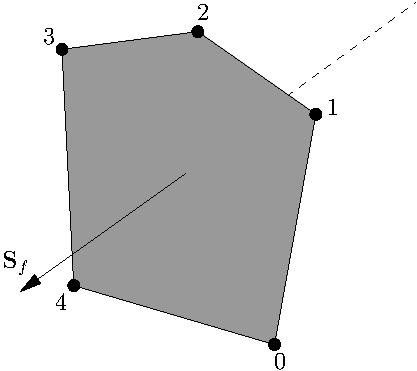
\includegraphics{fig-5-1}
 \caption{面における点の順序から決まる面領域ベクトル}
 \label{fig:5.1}
\end{figure}


面には2種類あります.
\begin{description}
 \item[内部の面]
            これらの面は必ず二つのセルに接続されており,
            その数が2を超えることはありません.
            また,内部の面において,その法線方向ベクトルが,
            より大きなラベルをもつセルに向くように,
            点のラベルの番号付けがなされます.
            つまり,セル2とセル5を接続している面だったら,
            その法線はセル5を向くわけです.
 \item[境界の面]
            これらは領域の境界にあるので,一つのセルにしか属しません.
            したがって,ある境界の面を参照するのは,
            一つのセルと境界パッチだけです.
            点ラベルの番号付けは,
            面の法線が計算領域の外側に向くように設定されます.
\end{description}

\subsubsection{セル}
\label{sssec:5.1.1.3}
セルは,面を任意の順序で並べたものです.セルは以下に示す性質が必ず必要です.
\begin{description}
 \item[切れ目なく連続である]
            セル群は計算領域全体を完全にカバーしており,
            かつ,お互いに重複してはなりません.
 \item[凸である]
            全てのセルは凸で,かつ,
            セル中心はセルの内側にある必要があります.
 \item[閉じている]
            全てのセルは幾何的にも位相的(トポロジ的)にも
            閉じていなければなりません.
            ここで,セルが幾何的に閉じているためには,
            全ての面領域ベクトルがセルの外側を向いているとして,
            それらのベクトル和が,正確にゼロ・ベクトルとなる必要があります.
            また,セルが位相的に閉じているためには,
            問題において,セル中の全ての辺が,
            二つの面により使用されている必要があります.
 \item[直交性がある]
            メッシュ内部の全ての面に対し,中心間ベクトルというのを,
            隣接する二つのセルの中心間を,
            小さいほうのラベルのセル中心から大きいほうのラベルの
            セル中心への向きで結んだベクトルとして定義することができます.
            直交性の制約というのは,内部の全ての面に対し,
            先に述べた面の面積ベクトルと中心間ベクトルのなす角が,
            常に$90\unit*{\degree}$未満であることをいいます.
\end{description}

\subsubsection{境界}
\label{sssec:5.1.1.4}
境界というのはパッチのリスト(集合)であり,
これら一つ一つは,ある境界条件が割り当てられています.
ここで,パッチというのは面のラベルのリストであり,
境界の面のみで形成され,内部の面を含みません.
この境界は閉じていることが条件であるので,
境界における全面領域ベクトルの和は,数値計算上ゼロ・ベクトルになります.


\subsection{\OFclass{polyMesh}の記述}
\label{ssec:5.1.2}
\OFpath{constant}ディレクトリのサブディレクトリである
\OFpath{polyMesh}には,
そのケースの
\index{polyMesh@\OFclass{polyMesh}!クラス}%
\index{クラス!polyMesh@\OFclass{polyMesh}}%
\OFclass{polyMesh}データが全て収められています.
このpolyMeshの記述は面ベースであり,既に述べましたように,
内部のセルは二つのセルと接続し,境界面はセルと境界のパッチを指定します.
各面には「保有」セルと「隣接」セルが割り当てられ,
面を通じた接続は,保有セルと隣接セルのラベルによって
簡潔に記述することができます.
境界の場合には,面に接続されたセルがその面の保有者であり,
隣接セルには$-1$のラベルが割り充てられます.
以上を踏まえた上で,以下のファイルで構成される入出力の詳細をご覧ください.
\begin{description}
 \item[\OFdictionary{points}]
\index{points@\OFdictionary{points}!ディクショナリ}%
\index{ディクショナリ!points@\OFdictionary{points}}%
            セルの頂点を記述するベクトルのリストです.
            ここで,リストにおける最初のベクトルは頂点$0$,
            次のベクトルの頂点$1$という風に番号付けします.
 \item[\OFdictionary{faces}]
\index{faces@\OFdictionary{faces}!ディクショナリ}%
\index{ディクショナリ!faces@\OFdictionary{faces}}%
            面のリストです.各面は点中の頂点の番号のリストで
            成り立ってます.ここで,先程と同様に,
            リスト中の最初の面の番号は$0$です.
 \item[\OFdictionary{owner}]
\index{owner@\OFdictionary{owner}!ディクショナリ}%
\index{ディクショナリ!owner@\OFdictionary{owner}}%
            保有セルのラベルのリストです.
            面のリストと同じ順番に並んでますので,
            リストの最初のラベルは$0$番の面の保有セルのラベル,
            次のラベルは$1$番の面の保有セルのラベルということになります.
 \item[\OFdictionary{neighbour}]
\index{neighbour@\OFdictionary{neighbour}!ディクショナリ}%
\index{ディクショナリ!neighbour@\OFdictionary{neighbour}}%
            隣接セルのラベルのリストです.
 \item[\OFdictionary{boundary}]
\index{boundary@\OFdictionary{boundary}!ディクショナリ}%
\index{ディクショナリ!boundary@\OFdictionary{boundary}}%
            パッチのリストです.以下のように,
            パッチ名の宣言で始まる各パッチに対するディクショナリで構成されます.
\begin{OFverbatim}[file]
movingWall
{
    type patch;
    nFaces 20;
    startFace 760;
}
\end{OFverbatim}
\index{startFace@\OFkeyword{startFace}!キーワード}%
\index{キーワード!startFace@\OFkeyword{startFace}}%
            \OFkeyword{startFace}はそのパッチにおける最初の面のラベル番号です.
            また
\index{nFaces@\OFkeyword{nFaces}!キーワード}%
\index{キーワード!nFaces@\OFkeyword{nFaces}}%
            \OFkeyword{nFaces}は,そのパッチ中の面数です.
\end{description}
備考:計算対象にいくつセルがあるか知りたい場合には,
\OFpath{owner}ファイルの\OFkeyword{FoamFile}ヘッダにおける
\OFkeyword{nCells}を見てください.


\subsection{\OFtool{cellShape}ツール}
\label{ssec:5.1.3}
標準的(でより単純)なメッシュ形式を,
OpenFOAMのライブラリで扱えるように変換する際に,
特に必要となるであろう\OFtool{cellShape}というツールについても説明しておきたいと思います.

多くのメッシュ・ジェネレータや後処理システムは,
実際にあり得る多面体セルの形状種類に対し,
その一部だけをサポートするものがほとんどです.
それらは,メッシュをセル形状セットといった,
3次元のセル幾何形状の限られた組み合わせで定義します.
OpenFOAMのライブラリには,
これらの一般的な形状集の定義がありますので,
上記のようなメッシュを先の節で述べたpolyMesh形式に変換することができます.

OpenFOAMによってサポートされるcellShapeモデルを
\autoref{tbl:5.1}に示します.
形状は,形状モデルにおける番号付けスキームに従って付けれらた
頂点ラベルの順序によって定義されます.
点や面,辺に対する番号付けスキームも\autoref{tbl:5.1}に書いてあります.
点の番号付けは,形状がねじれたり,
他の形状に変化することがないようにしなければならないので,
同じ点番号は複数回使用できないことになります.
さらに,重複した点はOpenFOAMでは使う必要はありません.
なぜなら,OpenFOAMで使用可能な形状は,六面体の変種を全てカバーしているからです.

セルの記述は,セルモデルの名前と,
ラベルの順序リストという二つの部分より行います.例えば,以下の点のリストを使うと,
\begin{OFverbatim}[file]
8
    (
        (0 0 0)
        (1 0 0)
        (1 1 0)
        (0 1 0)
        (0 0 0.5)
        (1 0 0.5)
        (1 1 0.5)
        (0 1 0.5)
    )
\end{OFverbatim}
六面体セルは以下のように書けます.
\begin{OFverbatim}[file]
(hex 8(0 1 2 3 4 5 6 7))
\end{OFverbatim}
ここで,六面体セルの形状は\OFkeyword{hex}というキーワードで記述しましたが,
他の形状については,\autoref{tbl:5.1}に示したキーワードを使って記述できます.


\begin{table}[p]
 %#! platex UserGuideJa
\begin{tabular}{llccc}
 セルタイプ & キーワード & 点の番号付け & 面の番号付け & 辺の番号付け \\
 \hline
 \tblstrut
 六面体 & \OFkeyword{hex}
     & 
\includegraphics{tbl-5-1-1-v}
         & 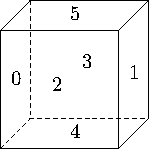
\includegraphics{tbl-5-1-1-f}
             & 
\includegraphics{tbl-5-1-1-e} \\
 くさび形 & \OFkeyword{wedge}
     & 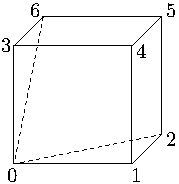
\includegraphics{tbl-5-1-2-v}
         & 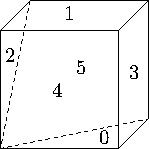
\includegraphics{tbl-5-1-2-f}
             & 
\includegraphics{tbl-5-1-2-e} \\
 三角柱 & \OFkeyword{prism}
     & 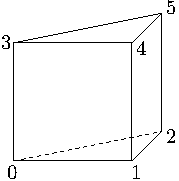
\includegraphics{tbl-5-1-3-v}
         & 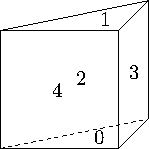
\includegraphics{tbl-5-1-3-f}
             & 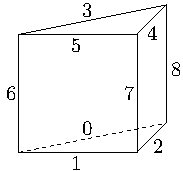
\includegraphics{tbl-5-1-3-e} \\
 四角錐 & \OFkeyword{pyr}
     & 
\includegraphics{tbl-5-1-4-v}
         & 
\includegraphics{tbl-5-1-4-f}
             & 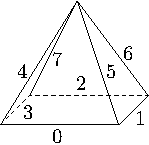
\includegraphics{tbl-5-1-4-e} \\
 四面体 & \OFkeyword{tet}
     & 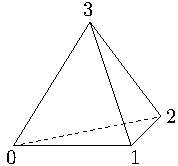
\includegraphics{tbl-5-1-5-v}
         & 
\includegraphics{tbl-5-1-5-f}
             & 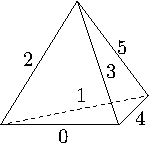
\includegraphics{tbl-5-1-5-e} \\
 くさび状四面体 & \OFkeyword{tetWedge}
     & 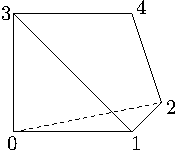
\includegraphics{tbl-5-1-6-v}
         & 
\includegraphics{tbl-5-1-6-f}
             & 
\includegraphics{tbl-5-1-6-e} \\
 \hline
\end{tabular}

 \caption{\OFtool{cellShapes}における頂点,面,辺の番号付け}
 \label{tbl:5.1}
\end{table}


\subsection{1次元や2次元,軸対称問題}
\label{ssec:5.1.4}
\index{1じげん@1次元!メッシュ}%
\index{メッシュ!1じげん@1次元}%
\index{2じげん@2次元!メッシュ}%
\index{メッシュ!2じげん@2次元}%
\index{1D!メッシュ}%
\index{メッシュ!1D}%
\index{2D!メッシュ}%
\index{メッシュ!2D}%
OpenFOAMは3次元の空間用に設計されており,
全てのメッシュもそのように定義します.
しかしながら,OpenFOAMでは,1次元や2次元
そして%
\index{じくたいしょう@軸対称!メッシュ}%
\index{メッシュ!じくたいしょう@軸対称}%
軸対称問題も解くことができ,
それには,法線方向が意図する方向であるパッチに対して,
特殊な境界条件を適用します.
具体的には,1次元や2次元問題では
\index{empty@\OFboundary{empty}!きょうかいじょうけん@境界条件}%
\index{きょうかいじょうけん@境界条件!empty@\OFboundary{empty}}%
\OFboundary{empty}のパッチタイプを使い,
軸対称問題では
\index{wedge@\OFboundary{wedge}!きょうかいじょうけん@境界条件}%
\index{きょうかいじょうけん@境界条件!wedge@\OFboundary{wedge}}%
\OFboundary{wedge}タイプを使います.
両者の使用法については\autoref{ssec:5.2.2}で触れ,
軸対称問題用の\OFkeyword{wedge}幾何形状の生成法については
\autoref{ssec:5.3.3}において述べます.



\section{境界}
\label{sec:5.2}
\index{きょうかい@境界}%
本節では境界について述べます.
境界はやや複雑です.なぜなら,形状の構成によって規定される
単純なものではなく,境界条件や境界間の接続を通して
解法を規定する不可欠の部分であるためです.
境界はメッシュ,物理量,離散化,計算法といった
多くの要素に関連しており,便宜上この章で扱います.

まず考えるべきことは,境界条件の適用のために,
境界は分割されてパッチの組み合わせになるということです.
一つのパッチは一つ以上の境界面に閉じられた領域をもち,
それらが物理的に接続している必要はありません.

下に階層を示すように,パッチに関する性質は3種類あり,
\autoref{fig:5.2}では各レベルにおけるさまざまな
パッチの名前を挙げています.
下で示す階層はOpenFOAMライブラリの階層構造と類似しています.
\begin{description}
 \item[Base type(基底型)]
            形状や情報の伝達を規定
 \item[Primitive type (基本型)]
            物理量の境界条件を規定
 \item[Derived type(派生型)]
            Primitive typeから派生した,複雑な境界条件を規定
\end{description}
\OFrevision{【要検討】baseとprimitiveの訳しかた}


\begin{figure}[ht]
 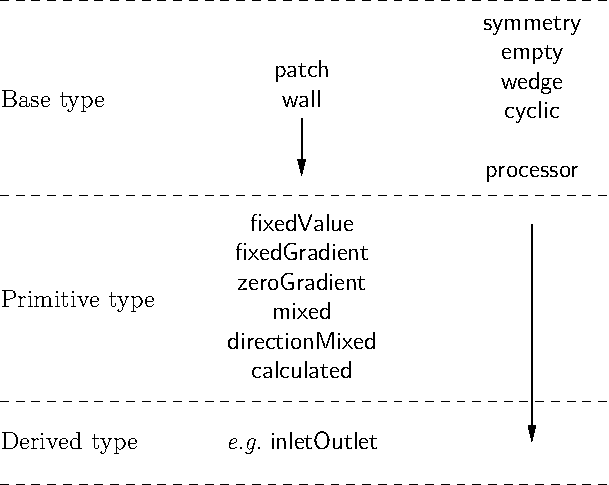
\includegraphics{fig-5-2}
 \caption{境界タイプの階層}
 \label{fig:5.2}
\end{figure}


\subsection{パッチの形式の類型化}
\label{ssec:5.2.1}
パッチの種類はメッシュと物理量のファイルに規定されます.
もう少し正確にいえば,
\begin{itemize}
 \item 基底型は\OFpath{constant/polyMesh}ディレクトリにある
       \OFpath{boundary}ファイル内の各パッチに対応する
\index{type@\OFkeyword{type}!キーワード}%
\index{キーワード!type@\OFkeyword{type}}%
       \OFkeyword{type}キーワードに従って記述されます.
 \item 数値パッチ型は,基本型または派生型となり,
       フィールドファイルの各パッチに対応する
\index{type@\OFkeyword{type}!キーワード}%
\index{キーワード!type@\OFkeyword{type}}%
       \OFkeyword{type}キーワードに従って記述されます.
\end{itemize}
例として\OFtool{sonicFoam}のケースにおける\OFpath{boundary}ファイルと
\OFpath{p}ファイル(圧力物理量ファイル)を示します.
\begin{OFverbatim}[file, linenum=17]

6
(
    inlet
    {
        type            patch;
        nFaces          50;
        startFace       10325;
    }
    outlet
    {
        type            patch;
        nFaces          40;
        startFace       10375;
    }
    bottom
    {
        type            symmetryPlane;
        nFaces          25;
        startFace       10415;
    }
    top
    {
        type            symmetryPlane;
        nFaces          125;
        startFace       10440;
    }
    obstacle
    {
        type            patch;
        nFaces          110;
        startFace       10565;
    }
    defaultFaces
    {
        type            empty;
        nFaces          10500;
        startFace       10675;
    }
)

// ************************************************************************* //
\end{OFverbatim}
\begin{OFverbatim}[file, linenum=17]
dimensions      [1 -1 -2 0 0 0 0];

internalField   uniform 1;

boundaryField
{
    inlet
    {
        type            fixedValue;
        value           uniform 1;
    }

    outlet
    {
        type            waveTransmissive;
        field           p;
        phi             phi;
        rho             rho;
        psi             psi;
        gamma           1.4;
        fieldInf        1;
        lInf            3;
        value           uniform 1;
    }

    bottom
    {
        type            symmetryPlane;
    }

    top
    {
        type            symmetryPlane;
    }

    obstacle
    {
        type            zeroGradient;
    }

    defaultFaces
    {
        type            empty;
    }
}

// ************************************************************************* //
\end{OFverbatim}
\OFpath{boundary}ファイルにおける\OFkeyword{type}は,
\OFkeyword{symmetryPlane}や\OFkeyword{empty}といった
幾何学的制約を受けるパッチを除くすべてのパッチに対して
\OFkeyword{patch}となっています.
\OFpath{p}ファイルには\OFkeyword{inlet}や
\OFkeyword{bottom}といった面に適用される基本型と
\OFkeyword{outlet}に適用される複雑な派生型が記述されています.
二つのファイルを比較すると,単純な\OFkeyword{patch}ではなく,
\OFkeyword{symmetryPlane}や\OFkeyword{empty}である場合,
基底型及び数値型で一致していることがわかります.


\subsection{ 基底型}
\label{ssec:5.2.2}
以下に基底型の種類を挙げます.
これらを規定するキーワードは\autoref{tbl:5.2}にまとめてあります.


\begin{figure}[ht]
 
\includegraphics{fig-5-3}
 \caption{\OFkeyword{wedge}パッチを利用した軸対象形状}
 \label{fig:5.3}
\end{figure}


\begin{table}[ht]
 %#! platex UserGuideJa
\begin{tabular}{ll}
 種類 & 意味 \\
 \hline
\index{patch@\OFkeyword{patch}!キーワードエントリ}%
\index{キーワードエントリ!patch@\OFkeyword{patch}}%
 \OFkeyword{patch} & 一般的なパッチ \\
\index{symmetryPlane@\OFkeyword{symmetryPlane}!キーワードエントリ}%
\index{キーワードエントリ!symmetryPlane@\OFkeyword{symmetryPlane}}%
 \OFkeyword{symmetryPlane} & 対称面 \\
\index{empty@\OFkeyword{empty}!キーワードエントリ}%
\index{キーワードエントリ!empty@\OFkeyword{empty}}%
 \OFkeyword{empty} & 2次元形状の前後の面 \\
\index{wedge@\OFkeyword{wedge}!キーワードエントリ}%
\index{キーワードエントリ!wedge@\OFkeyword{wedge}}%
 \OFkeyword{wedge} & 軸対称形状のための,くさび型の前後 \\
\index{cyclic@\OFkeyword{cyclic}!キーワードエントリ}%
\index{キーワードエントリ!cyclic@\OFkeyword{cyclic}}%
 \OFkeyword{cyclic} & 周期境界面 \\
\index{wall@\OFkeyword{wall}!キーワードエントリ}%
\index{キーワードエントリ!wall@\OFkeyword{wall}}%
 \OFkeyword{wall} & 壁面(乱流の壁関数に使用) \\
\index{processor@\OFkeyword{processor}!キーワードエントリ}%
\index{キーワードエントリ!processor@\OFkeyword{processor}}%
 \OFkeyword{processor} & 並列計算時のプロセッサ間の境界 \\
 \hline
\end{tabular}

 \caption{基底型の境界の種類}
 \label{tbl:5.2}
\end{table}


\begin{description}
 \item[\OFboundary{patch}]
\index{patch@\OFboundary{patch}!きょうかいじょうけん@境界条件}%
\index{きょうかいじょうけん@境界条件!patch@\OFboundary{patch}}%
            メッシュに対する形状的,
            位相的情報をなにももたないパッチ条件のための
            基礎的なパッチ (\OFkeyword{wall}の場合を除く).
            流入口や流出口など.
 \item[\OFboundary{wall}]
\index{wall@\OFboundary{wall}!きょうかいじょうけん@境界条件}%
\index{きょうかいじょうけん@境界条件!wall@\OFboundary{wall}}%
            特に専門家が壁の境界を規定するときに,
            壁に適合するパッチが以下のように
            特定可能である必要がある場合があります.
            良い例としては,壁が\OFkeyword{wall}パッチの型で
            特定されなければならない壁乱流モデルがあり,
            壁に隣接するセルの中心からの距離がパッチの一部として格納されます.
 \item[\OFboundary{symmetryPlane}]
\index{symmetryPlane@\OFboundary{symmetryPlane}!きょうかいじょうけん@境界条件}%
\index{きょうかいじょうけん@境界条件!symmetryPlane@\OFboundary{symmetryPlane}}%
            対称面
 \item[\OFboundary{empty}]
\index{empty@\OFboundary{empty}!きょうかいじょうけん@境界条件}%
\index{きょうかいじょうけん@境界条件!empty@\OFboundary{empty}}%
            OpenFOAMが常に3次元で形状を生成する一方で,
            2次元(1次元)を解くことも可能です.
            そのためには,解が必要とされない3番目(2番目)の次元に
            法線が向いている各パッチに特別な\OFkeyword{empty}条件を当てはめます.
 \item[\OFboundary{wedge}]
\index{wedge@\OFboundary{wedge}!きょうかいじょうけん@境界条件}%
\index{きょうかいじょうけん@境界条件!wedge@\OFboundary{wedge}}%
            シリンダのような2次元の%
\index{じくたいしょう@軸対称!もんだい@問題}%
            軸対称問題では,
            \autoref{fig:5.3}で示すように,
            小さい角度 (例えば$< 5\unit*{\degree}$) のくさびで,
            座標面の一つにまたがる対称面に沿って伸びている
            一つのセルとして形状が記述されます.
            軸対称くさび面は\OFkeyword{wedge}型という独自のパッチである必要があります.
            \OFtool{blockMesh}を使ったくさびの形状の生成に関する詳細は
            \autoref{ssec:5.3.3}に述べられています.
 \item[\OFboundary{cyclic}]
\index{cyclic@\OFboundary{cyclic}!きょうかいじょうけん@境界条件}%
\index{きょうかいじょうけん@境界条件!cyclic@\OFboundary{cyclic}}%
            熱交換管のような繰り返しの多い形状では,
            二つのパッチをあたかも一つのように扱うことができるようにする場合があります.
            ある\OFboundary{cyclic}パッチは
            \OFpath{boundary}ファイル内の\OFkeyword{neighbourPatch}キーワードで
            もう一つのパッチと結び付けられます.
            接続される面の各ペアは,
            \OFpath{boundary}ファイル内の\OFkeyword{matchTolerance}キーワードで
            与えられる許容誤差に収まるような,ほぼ等しい面積をもっている必要があります.
            面の方向が一致している必要はありません.
 \item[\OFboundary{processor}]
\index{processor@\OFboundary{processor}!きょうかいじょうけん@境界条件}%
\index{きょうかいじょうけん@境界条件!processor@\OFboundary{processor}}%
            多数のプロセッサで計算を並列実行する際には,
            各プロセッサがほぼ同数のセルを計算するようにメッシュを分割する必要があります.
            別々のメッシュの間の境界は\OFkeyword{processor}境界とよばれます.
\end{description}


\subsection{基本型}
\label{ssec:5.2.3}
\autoref{tbl:5.3}に基本型の種類を挙げます.


\begin{table}[ht]
 %#! platex UserGuideJa
\begin{tabularx}{\textwidth}{lXp{8zw}}
 種類 & 物理量$\phi$に対して与える条件 & Data to specify \\
 \hline
\index{fixedValue@\string\OFboundary{fixedValue}!きょうかいじょうけん@境界条件}%
\index{きょうかいじょうけん@境界条件!fixedValue@\string\OFboundary{fixedValue}}%
 \OFboundary{fixedValue} & $\phi$の値が一定 & \OFkeyword{value} \\
\index{fixedGradient@\string\OFboundary{fixedGradient}!きょうかいじょうけん@境界条件}%
\index{きょうかいじょうけん@境界条件!fixedGradient@\string\OFboundary{fixedGradient}}%
 \OFboundary{fixedGradient} & $\phi$の勾配が一定 & \OFkeyword{gradient} \\
\index{zeroGradient@\string\OFboundary{zeroGradient}!きょうかいじょうけん@境界条件}%
\index{きょうかいじょうけん@境界条件!zeroGradient@\string\OFboundary{zeroGradient}}%
 \OFboundary{zeroGradient} & $\phi$の勾配が$0$ & -- \\
\index{calculated@\string\OFboundary{calculated}!きょうかいじょうけん@境界条件}%
\index{きょうかいじょうけん@境界条件!calculated@\string\OFboundary{calculated}}%
 \OFboundary{calculated} & $\phi$の境界条件が他の物理量から決まる & -- \\
\index{mixed@\string\OFboundary{mixed}!きょうかいじょうけん@境界条件}%
\index{きょうかいじょうけん@境界条件!mixed@\string\OFboundary{mixed}}%
 \OFboundary{mixed} & \OFboundary{fixedValue}と\OFboundary{fixedGradient}の組み合わせ,
     \OFkeyword{valueFraction}に依存する条件 &
         \OFkeyword{refValue},\hfil\break
\index{refGradient@\string\OFkeyword{refGradient}!キーワード}%
\index{キーワード!refGradient@\string\OFkeyword{refGradient}}%
         \OFkeyword{refGradient},\hfil\break
\index{valueFraction@\string\OFkeyword{valueFraction}!キーワード}%
\index{キーワード!valueFraction@\string\OFkeyword{valueFraction}}%
         \OFkeyword{valueFraction},\hfil\break
\index{value@\string\OFkeyword{value}!キーワード}%
\index{キーワード!value@\string\OFkeyword{value}}%
         \OFkeyword{value} \\
\index{directionMixed@\string\OFboundary{directionMixed}!きょうかいじょうけん@境界条件}%
\index{きょうかいじょうけん@境界条件!directionMixed@\string\OFboundary{directionMixed}}%
 \OFboundary{directionMixed} &
     \OFrevision*{要再訳}%
     例えば法線方向と接線方向の異なるレベルでの組み合わせのような,
     テンソルの\OFkeyword{valueFraction}に対しては\OFkeyword{mixed}条件 &
         \OFkeyword{refValue},\hfil\break
         \OFkeyword{refGradient},\hfil\break
         \OFkeyword{valueFraction},\hfil\break
         \OFkeyword{value} \\
 \hline
\end{tabularx}

 \caption{基本型のパッチの種類}
 \label{tbl:5.3}
\end{table}


\subsection{派生型}
\label{ssec:5.2.4}
OpenFOAMには多数の派生型境界条件があり,ここには掲載しきれません.
かわりに,ごく一部を\autoref{tbl:5.4}に紹介します.
利用できる全てのモデルの一覧を得たければ,
OpenFOAMのソースコードを参照してください.
派生型境界条件のソースコードは以下のような場所にあります.
\begin{itemize}
 \item \OFpath{\$FOAM SRC/finiteVolume/fields/fvPatchFields/derived}の中
 \item 特定のモデルライブラリの中.
       ターミナルで以下のようなコマンドを実行することで探せます.
\begin{OFverbatim}{terminal}
find $FOAM_SRC -name "*derivedFvPatch*"
\end{OFverbatim}%$
 \item 特定のソルバの中.
       ターミナルで以下のようなコマンドを実行することで探せます.
\begin{OFverbatim}{terminal}
find $FOAM_SOLVERS -name "*fvPatch*"
\end{OFverbatim}%$
\end{itemize}



\begin{table}[p]
 \rotatebox{90}{%
 \small
 \begin{minipage}{\textheight}
  %#! platex UserGuideJa
\begin{tabularx}{\textheight}{lXp{9zw}}
 \OFboundary{fixedValue}から派生 & 意味 & 指定するデータ \\
 \hline
\index{movingWallVelocity@\string\OFboundary{movingWallVelocity}!きょうかいじょうけん@境界条件}%
\index{きょうかいじょうけん@境界条件!movingWallVelocity@\string\OFboundary{movingWallVelocity}}%
 \OFboundary{movingWallVelocity} &
     ノーマルパッチの値を置き換えるのでパッチのフラックスは$0$ & \OFkeyword{value} \\
\index{pressureInletVelocity@\string\OFboundary{pressureInletVelocity}!きょうかいじょうけん@境界条件}%
\index{きょうかいじょうけん@境界条件!pressureInletVelocity@\string\OFboundary{pressureInletVelocity}}%
 \OFboundary{pressureInletVelocity} &
     流入口の$p$が分かっているとき,$\bm{U}$は,フラックスから評価され,
     パッチはノーマル. & \OFkeyword{value} \\
\index{pressureDirectedInletVelocity@\string\OFboundary{pressureDirectedInletVelocity}!きょうかいじょうけん@境界条件}%
\index{きょうかいじょうけん@境界条件!pressureDirectedInletVelocity@\string\OFboundary{pressureDirectedInletVelocity}}%
 \OFboundary{pressureDirectedInletVelocity} &
     流入口の$p$が分かっているとき,$\bm{U}$は,
     \OFkeyword{inletDirection}のフラックスから計算される. &
         \OFkeyword{value},\OFkeyword{inletDirection} \\
\index{surfaceNormalFixedValue@\string\OFboundary{surfaceNormalFixedValue}!きょうかいじょうけん@境界条件}%
\index{きょうかいじょうけん@境界条件!surfaceNormalFixedValue@\string\OFboundary{surfaceNormalFixedValue}}%
 \OFboundary{surfaceNormalFixedValue} &
     大きさによって,ベクトル境界条件をノーマルパッチに指定します.
     ベクトルの+veはドメインを指す. & \OFkeyword{value} \\
\index{totalPressure@\string\OFboundary{totalPressure}!きょうかいじょうけん@境界条件}%
\index{きょうかいじょうけん@境界条件!totalPressure@\string\OFboundary{totalPressure}}%
 \OFboundary{totalPressure} &
     全圧$p_{0} = p + \frac{1}{2}\rho|\bm{U}|^{2}$は固定.
     $\bm{U}$が変わるとそれに従い$p$も調整される. & \OFkeyword{p0} \\
\index{turbulentInlet@\string\OFboundary{turbulentInlet}!きょうかいじょうけん@境界条件}%
\index{きょうかいじょうけん@境界条件!turbulentInlet@\string\OFboundary{turbulentInlet}}%
 \OFboundary{turbulentInlet} &
     平均値のスケールに基づく変動変数について計算する &
         \OFkeyword{referenceField}, \OFkeyword{fluctuationScale} \\
 \\
 \OFboundary{fixedGradient}/\OFboundary{zeroGradient}から派生 \\
 \hline
\index{fluxCorrectedVelocity@\string\OFboundary{fluxCorrectedVelocity}!きょうかいじょうけん@境界条件}%
\index{きょうかいじょうけん@境界条件!fluxCorrectedVelocity@\string\OFboundary{fluxCorrectedVelocity}}%
 \OFboundary{fluxCorrectedVelocity} &
     フラックスから流入口の$\bm{U}$の法線成分を計算する &
         \OFkeyword{value} \\
\index{wallBuoyantPressure@\string\OFboundary{wallBuoyantPressure}!きょうかいじょうけん@境界条件}%
\index{きょうかいじょうけん@境界条件!wallBuoyantPressure@\string\OFboundary{wallBuoyantPressure}}%
 \OFboundary{wallBuoyantPressure} &
     気圧勾配に基づく\OFboundary{fixedGradient}圧を設定する & --- \\
 \\
 \OFboundary{mixed}から派生 \\
 \hline
\index{inletOutlet@\string\OFboundary{inletOutlet}!きょうかいじょうけん@境界条件}%
\index{きょうかいじょうけん@境界条件!inletOutlet@\string\OFboundary{inletOutlet}}%
 \OFboundary{inletOutlet} &
     $\bm{U}$の向きによって\OFboundary{fixedValue}と
     \OFboundary{zeroGradient}の間で$\bm{U}$と$p$を切り替える &
         \OFkeyword{inletValue},\OFkeyword{value} \\
\index{outletInlet@\string\OFboundary{outletInlet}!きょうかいじょうけん@境界条件}%
\index{きょうかいじょうけん@境界条件!outletInlet@\string\OFboundary{outletInlet}}%
 \OFboundary{outletInlet} &
     $\bm{U}$の向きによって\OFboundary{fixedValue}と
     \OFboundary{zeroGradient}の間で$\bm{U}$と$p$を切り替える &
         \OFkeyword{outletValue},\OFkeyword{value} \\
 \OFboundary{pressureInletOutletVelocity} &
     \OFboundary{pressureInletVelocity}と
     \OFboundary{inletOutlet}の組み合わせ & \OFkeyword{value} \\
 \OFboundary{pressureDirectedInletOutletVelocity} &
     \OFboundary{pressureDirectedInletVelocity}と\OFboundary{inletOutlet}の組み合わせ &
         \OFkeyword{value},\OFkeyword{inletDirection} \\
\index{pressureTransmissive@\string\OFboundary{pressureTransmissive}!きょうかいじょうけん@境界条件}%
\index{きょうかいじょうけん@境界条件!pressureTransmissive@\string\OFboundary{pressureTransmissive}}%
 \OFboundary{pressureTransmissive} &
     周囲の圧力$p_{\infty}$に超音速圧縮波を伝える & \OFkeyword{pInf} \\
\index{supersonicFreeStream@\string\OFboundary{supersonicFreeStream}!きょうかいじょうけん@境界条件}%
\index{きょうかいじょうけん@境界条件!supersonicFreeStream@\string\OFboundary{supersonicFreeStream}}%
 \OFboundary{supersonicFreeStream} &
     斜めの衝撃を$p_{\infty}$,$T_{\infty}$,$U_{\infty}$の環境に伝える &
         \OFkeyword{pInf},\OFkeyword{TInf},\OFkeyword{UInf} \\
 その他 \\
 \hline
\index{slip@\string\OFboundary{slip}!きょうかいじょうけん@境界条件}%
\index{きょうかいじょうけん@境界条件!slip@\string\OFboundary{slip}}%
 \OFboundary{slip} & $\phi$がスカラなら\OFboundary{zeroGradient},
     $\phi$がベクトルなら法線成分は\OFboundary{fixedValue 0}で,
     接線成分は\OFboundary{zeroGradient} & --- \\
\index{partialSlip@\string\OFboundary{partialSlip}!きょうかいじょうけん@境界条件}%
\index{きょうかいじょうけん@境界条件!partialSlip@\string\OFboundary{partialSlip}}%
 \OFboundary{partialSlip} &
     混合\OFboundary{zeroGradient}/\OFboundary{slip}条件は
     \OFkeyword{valueFraction}による.\OFboundary{slip}ならば$1$. &
         \OFkeyword{valueFraction} \\
 \hline
\end{tabularx}

  Note: $p$は圧力, $\bm{U}$は速度
  \caption{派生型の種類}
  \label{tbl:5.4}
 \end{minipage}}
\end{table}



\section{\OFtool{blockMesh}ユーティリティを使ったメッシュ生成}
\label{sec:5.3}
\index{blockMesh@\OFtool{blockMesh}!ユーティリティ}%
\index{ユーティリティ!blockMesh@\OFtool{blockMesh}}%
\index{メッシュ!せいせい@生成}%
本節では,OpenFOAM付属の
メッシュ生成ユーティリティの\OFtool{blockMesh}について説明します.
\OFtool{blockMesh}ユーティリティは,
\index{メッシュ!こうばいづけ@勾配付け}%
勾配付けや曲がった辺を使ったパラメトリックなメッシュを作成します.

メッシュはケースの\OFpath{constant/polyMesh}ディレクトリに位置する
\index{blockMeshDict@\OFdictionary{blockMeshDict}!ディクショナリ}%
\index{ディクショナリ!blockMeshDict@\OFdictionary{blockMeshDict}}%
\OFdictionary{blockMeshDict}というディクショナリファイルから生成します.
\OFtool{blockMesh}はこのディクショナリを読み込んでメッシュを生成し,
同じディレクトリの
\index{points@\OFdictionary{points}!ディクショナリ}%
\index{ディクショナリ!points@\OFdictionary{points}}%
\OFdictionary{points},
\index{faces@\OFdictionary{faces}!ディクショナリ}%
\index{ディクショナリ!faces@\OFdictionary{faces}}%
\OFdictionary{faces},
\index{cells@\OFdictionary{cells}!ディクショナリ}%
\index{ディクショナリ!cells@\OFdictionary{cells}}%
\OFdictionary{cells}および
\index{boundary@\OFdictionary{boundary}!ディクショナリ}%
\index{ディクショナリ!boundary@\OFdictionary{boundary}}%
\OFdictionary{boundary}ファイルに
メッシュ・データを書き出します.

\OFtool{blockMesh}がよりどころとする原則は,
一つあるいは複数の3次元の六面体のブロックに領域を分割することです.
ブロックの辺は,直線,円弧またはスプラインであるかもしれません.
メッシュは,ブロックの各方向の多くのセルとして表面上指定され,
これは\OFtool{blockMesh}がメッシュ・データを生成するのに必要な情報です.

各ブロックの幾何形状は八つの頂点,
六面体の各隅のひとつによって定義されます.
頂点はリストの中に書かれ,各頂点にはそのラベルでアクセスできるようになっています.
OpenFOAMは常にC++の慣習に従って,
リストの最初の要素をラベル `0' とします.
リストに従って,各頂点に番号付けがされているブロックの例を
\autoref{fig:5.5}に示します.
頂点1と5を接続する辺をみてわかるように,
\OFtool{blockMesh}では曲線を作ることもできます.

\autoref{ssec:5.3.3}で説明するように,
1組以上の頂点をお互いに重ねることで
八つ未満の頂点をもつブロックを生成することも可能です.

各ブロックは,
\index{ざひょうじく@座標軸!みぎてけい@右手系}
右手系である局所座標系$(x_{1}, x_{2}, x_{3})$をもちます.
右手系の軸群は,$Oz$軸を見下ろしたとき,
$Ox$軸上の点から$Oy$軸上への円弧が時計回りとなるように定義されます.
局所座標系は以下に従ってブロックの定義で提示された
頂点の順序に従って定義されます.
\begin{itemize}
 \label{p:U-130}
 \item 軸の原点はブロックの定義における最初の入力です.
       例では頂点0です.
 \item $x_{1}$の方向は,頂点0から頂点1まで動くことによって示されます.
 \item $x_{2}$の方向は,頂点1から頂点2まで動くことによって示されます.
 \item 頂点0,1,2,3は$x_{3} = 0$の平面を定義します.
 \item 頂点4は頂点0から$x_{3}$方向へ辿っていくと見つかります.
 \item 頂点5,6,および7は,頂点1,2,および3から
       それぞれ$x_{3}$の方向へ辿っていくことで,同様に見つかります.
\end{itemize}


\begin{figure}[ht]
 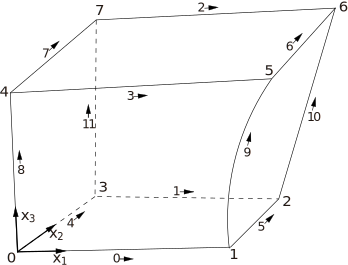
\includegraphics{fig-5-5}
 \caption{ひとつのブロック}
 \label{fig:5.5}
\end{figure}


\begin{table}[ht]
 %#! platex UserGuideJa
\begin{tabularx}{\textwidth}{lXX}
 キーワード & 説明 & 指定するデータ \\
 \hline
\index{convertToMeters@\string\OFkeyword{convertToMeters}!キーワード}%
\index{キーワード!convertToMeters@\string\OFkeyword{convertToMeters}}%
 \OFkeyword{convertToMeters} &
     頂点座標の倍率 &
         \OFkeyword{0.001}とすれば$\unit*{mm}$ \\
\index{vertices@\string\OFkeyword{vertices}!キーワード}%
\index{キーワード!vertices@\string\OFkeyword{vertices}}%
 \OFkeyword{vertices} &
     頂点座標のリスト &
         \OFkeyword{(0 0 0)} \\
\index{edges@\string\OFkeyword{edges}!キーワード}%
\index{キーワード!edges@\string\OFkeyword{edges}}%
 \OFkeyword{edges} &
\index{arc@\string\OFkeyword{arc}!キーワード}%
\index{キーワード!arc@\string\OFkeyword{arc}}%
     \OFkeyword{arc}もしくは
\index{spline@\string\OFkeyword{spline}!キーワード}%
\index{キーワード!spline@\string\OFkeyword{spline}}%
     \OFkeyword{spline}の辺を書くために使用 &
         arc 1 4 (0.939 0.342 -0.5) \\
\index{block@\string\OFkeyword{block}!キーワード}%
\index{キーワード!block@\string\OFkeyword{block}}%
 \OFkeyword{block} &
     頂点ラベルとメッシュサイズの順序リスト &
         \OFkeyword{hex (0 1 2 3 4 5 6 7)}\par
         \OFkeyword{(10 10 1)}\par
         \mbox{\OFkeyword{simpleGrading (1.0 1.0 1.0)}} \\
\index{patches@\string\OFkeyword{patches}!キーワード}%
\index{キーワード!patches@\string\OFkeyword{patches}}%
 \OFkeyword{patches} &
     パッチのリスト &
         \OFkeyword{symmetryPlane base}\par
         \OFkeyword{( (0 1 2 3) )} \\
\index{mergePatchPairs@\string\OFkeyword{mergePatchPairs}!キーワード}%
\index{キーワード!mergePatchPairs@\string\OFkeyword{mergePatchPairs}}%
 \OFkeyword{mergePatchPairs} &
     マージするパッチのリスト &
         \autoref{ssec:5.3.2}参照 \\
 \hline
\end{tabularx}

 \caption{\OFdictionary{blockMeshDict}に使用するキーワード}
 \label{tbl:5.5}
\end{table}


\subsection{\OFdictionary{blockMeshDict}ファイルの記述}
\label{ssec:5.3.1}
\OFdictionary{blockMeshDict}ファイルは,
\autoref{tbl:5.5}で説明されている
キーワードを使用するディクショナリです.
\index{convertToMeters@\OFkeyword{convertToMeters}!キーワード}%
\index{キーワード!convertToMeters@\OFkeyword{convertToMeters}}%
\OFkeyword{convertToMeters}キーワードは,
メッシュ記述におけるすべての頂点の座標にかけられる
尺度因子を指定します.例えば,
\begin{OFverbatim}[file]
convertToMeters 0.001;
\end{OFverbatim}
は,すべての座標に$0.001$をかけることを意味します.
すなわち,\OFdictionary{blockMeshDict}ファイルで引用された値が$\unit*{mm}$になります.

\subsubsection{頂点}
\label{sssec:5.3.1.1}
メッシュのブロックの頂点は,
\OFkeyword{vertices}と名づけられた
標準のリストとして以下のように与えられます.
例えば\autoref{fig:5.5}での私たちの例のブロックに関しては,
頂点は以下のとおりです.
\begin{OFverbatim}[file]
vertices
(
    ( 0 0 0 ) // vertex number 0
    ( 1 0 0.1) // vertex number 1
    ( 1.1 1 0.1) // vertex number 2
    ( 0 1 0.1) // vertex number 3
    (-0.1 -0.1 1 ) // vertex number 4
    ( 1.3 0 1.2) // vertex number 5
    ( 1.4 1.1 1.3) // vertex number 6
    ( 0 1 1.1) // vertex number 7
);
\end{OFverbatim}

\subsubsection{辺}
\label{sssec:5.3.1.2}
2頂点をつなぐ各辺はデフォルトで直線とみなされます.
ただし,\OFkeyword{edges}というリスト内のエントリで,
いずれの辺も曲線として指定することができます.
このリストはオプションです.
ジオメトリ内に曲線が一つもなければ省略できます.

曲線の各エントリは,
\autoref{tbl:5.6}に挙げられているものから
カーブのタイプを指定するキーワードとともに始まります.


\begin{table}[ht]
 %#! platex UserGuideJa
\begin{tabular}{lll}
 キーワード選択 & 説明 & 追加するエントリ \\
 \hline
\index{arc@\OFkeyword{arc}!キーワードエントリ}%
\index{キーワードエントリ!arc@\OFkeyword{arc}}%
 \OFkeyword{arc} & 円弧 & 1点の補間点 \\
\index{simpleSpline@\OFkeyword{simpleSpline}!キーワードエントリ}%
\index{キーワードエントリ!simpleSpline@\OFkeyword{simpleSpline}}%
 \OFkeyword{simpleSpline} & スプライン曲線 & 補間点リスト \\
\index{polyLine@\OFkeyword{polyLine}!キーワードエントリ}%
\index{キーワードエントリ!polyLine@\OFkeyword{polyLine}}%
 \OFkeyword{polyLine} & 線群 & 補間点リスト \\
\index{polySpline@\OFkeyword{polySpline}!キーワードエントリ}%
\index{キーワードエントリ!polySpline@\OFkeyword{polySpline}}%
 \OFkeyword{polySpline} & スプライン群 & 補間点リスト \\
\index{line@\OFkeyword{line}!キーワードエントリ}%
\index{キーワードエントリ!line@\OFkeyword{line}}%
 \OFkeyword{line} & 直線 & --- \\
 \hline
\end{tabular}

 \caption{\OFdictionary{blockMeshDict}ディクショナリで使用可能なエッジタイプ}
 \label{tbl:5.6}
\end{table}


そして,キーワードの後には辺が接続する二つの頂点のラベルが続きます.
それに続いて,辺が通り過ぎる内挿点を指定しなければなりません.
\OFkeyword{arc}には,円弧が横切ることになる一つの内挿点が必要です.
\OFkeyword{simpleSpline},\OFkeyword{polyLine},
および\OFkeyword{polySpline}に関しては,内挿点のリストが必要です.
\OFkeyword{line}辺は,デフォルトとして実行されるオプションと
全く同等であり,内挿点を全く必要としません.
\OFkeyword{line}辺を使用する必要は全くありませんが,
それが完全性のために含まれていることに注意してください.
\autoref{fig:5.6}に示した例題のブロックでは,
内挿点$(1.1, 0.0, 0.5)$を通して以下のように
頂点1と5をつなぐ\OFkeyword{arc}辺を指定します.
\begin{OFverbatim}[file]
edges
(
    arc 1 5 (1.1 0.0 0.5)
);
\end{OFverbatim}

\subsubsection{ブロック}
\label{sssec:5.3.1.3}
ブロックの定義は
\index{blocks@\OFkeyword{blocks}!キーワード}%
\index{キーワード!blocks@\OFkeyword{blocks}}%
\OFkeyword{blocks}と名づけられたリストに含まれています.
各ブロックの定義は,\autoref{sec:5.3}で示された順序をもつ
頂点ラベルのリストからなる複合入力です.
ベクトルが各方向に必要なセルの数,タイプ,
および各方向のセル拡大比のリストを与えます.

そして,ブロックは以下のとおり定義されます.
\begin{OFverbatim}[file]
blocks
(
    hex (0 1 2 3 4 5 6 7) // vertex numbers
    (10 10 10) // numbers of cells in each direction
    simpleGrading (1 2 3) // cell expansion ratios
);
\end{OFverbatim}
それぞれのブロックの定義は以下のとおりです.
\begin{description}
 \item[Vertex numbering]
\index{blockMesh@\OFtool{blockMesh}!じっこうかのう@実行可能な頂点の番号付け}%
            \OFpath{OpenFOAM-2.0.0/cellModels}ファイルに
            定義されているように,最初の入力がブロックの
\index{けいじょう@形状}%
            形状識別子です.
            いつもブロックが六面体であるので,
            いつも形は\OFkeyword{hex}です.
            \pageref{p:U-130}ページで説明された方法で並べられた
            頂点番号のリストが従います.
 \item[Number of cells]
            2番目の入力はそのブロックの$x_{1}$,$x_{2}$,$x_{3}$と
            それぞれの方向のセルの数を与えます.
 \item[Cell expansion ratios]
\index{ブロック!かくだいりつ@拡大率}%
\index{セル!かくだいりつ@拡大率}%
            3番目の入力はブロックにおける各方向へのセルの拡大比を与えます.
            拡大比は,メッシュが指定された方向に段階的なものにするか,
            または精製されるのを可能にします.
            比率$\delta_{\mathrm{e}}$は\autoref{fig:5.6}に示すように,
            ブロックのひとつの辺に沿った終わりのセルの幅の,
            辺に沿った始めのセル幅$\delta_{\mathrm{s}}$への比です.
            以下のキーワードのそれぞれは\OFtool{blockMesh}で利用可能な
\index{メッシュ!こうばいづけ@勾配付け}%
            勾配付けの仕様の二つのタイプの一つを指定します.
            \begin{description}
             \item[simpleGrading]
\index{simpleGrading@\OFkeyword{simpleGrading}!キーワード}%
\index{キーワード!simpleGrading@\OFkeyword{simpleGrading}}%
                        簡単な記述で,局所的な$x_{1}$,$x_{2}$と$x_{3}$方向それぞれに一様な
                        拡大比を,三つの拡大比だけで指定します.例えば
\begin{OFverbatim}[file]
simpleGrading (1 2 3)
\end{OFverbatim}
             \item[edgeGrading]
\index{edgeGrading@\OFkeyword{edgeGrading}!キーワード}%
\index{キーワード!edgeGrading@\OFkeyword{edgeGrading}}%
                        完全なセルの拡大比の記述は,
                        \autoref{fig:5.5}に矢印で
                        「最初のセルから最後のセル」の方向を表した
                        スキームに従って番号付けられた
                        ブロックの各辺に比率を与えます.
                        例えば,このようなものです.
\begin{OFverbatim}[file]
edgeGrading (1 1 1 1 2 2 2 2 3 3 3 3)
\end{OFverbatim}
                        これは,辺$0$--$3$に沿ったセル幅の比率が$1$,
                        辺$4$--$7$に沿った比率が$2$であり,
                        辺$8$--$11$に沿った比率が$3$である
                        ということであることを意味しており,
                        上述した\OFkeyword{simpleGrading}の例に
                        まったく同等です.
            \end{description}
\end{description}


\begin{figure}[ht]
 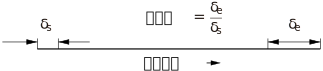
\includegraphics{fig-5-6}
 \caption{ブロックの辺に沿って段階わけされたメッシュ}
 \label{fig:5.6}
\end{figure}


\subsubsection{境界}
\label{sssec:5.3.1.4}
\index{boundary@\OFkeyword{boundary}!キーワード}%
\index{キーワード!boundary@\OFkeyword{boundary}}%
\index{boundary keyword@\OFtool{boundary keyword}}%
\OFkeyword{boundary}というリストでメッシュの境界を与えます.
境界はパッチ(領域)に分解され,
リストされた各パッチは名前をキーワードとしてもっています.
この名前はユーザが決めますが,例えば\OFkeyword{inlet}のように
そのパッチの意味がわかりやすいような名前にすることをお勧めします.
フィールドのデータファイルで境界条件を設定するときの識別にも,この名前が使われます.
パッチの情報は以下のサブディクショナリ内に収められます.
\begin{itemize}
 \item \OFkeyword{type}:
       パッチタイプ.
       適用できる境界条件がいくつかある一般的な\OFkeyword{patch}か,
       あるいは\autoref{tbl:5.1}にリストアップされ
       \autoref{ssec:5.2.2}で説明している特殊な幾何的条件のどちらか.
 \item \OFkeyword{faces}:
       パッチを作るブロックの面のリスト.
       名前はユーザの選択に任されますが
       例えば\OFkeyword{inlet}のように,
       パッチの特定に便利な名前を推奨します.
       この名前は,境界条件をフィールドのデータファイルに
       設定する際の識別に使用されます.
\end{itemize}
\OFtool{blockMesh}は\OFkeyword{boundary}リストに含まれない全ての面を集めて,
それらに\OFkeyword{defaultFaces}という名前で
\OFkeyword{empty}タイプのデフォルトパッチを割り当てます.
これは,2次元の幾何形状において,
それらが必要に応じて\OFkeyword{empty}パッチに
集められるのを知りながら,
ユーザは2次元平面にあるブロック面を
省略する選択ができることを意味します.

\autoref{fig:5.5}での例のブロックに戻って,
もし左面に流入があり,右面における流出があり,
他の四つの表面が壁であるならば,以下のとおりパッチは定義できるでしょう.
\begin{OFverbatim}[file]
boundary               // keyword
(
    inlet              // patch name
    {
        type patch;    // patch type for patch 0
        faces
        (
            (0 4 7 3)  // block face in this patch
        );
    }                  // end of 0th patch definition

    outlet             // patch name
    {
        type patch;    // patch type for patch 1
        faces
        (
            (1 2 6 5)
        );
    }

    walls
    {
        type wall;
        faces
        (
            (0 1 5 4)
            (0 3 2 1)
            (3 7 6 2)
            (4 5 6 7)
        );
    }
);
\end{OFverbatim}
それぞれのブロック面は四つの頂点番号のリストによって定義されます.
頂点が与えられる順序は,ブロックの中から見て,
どの頂点からも始めても,他の頂点を定義するために
時計回りに面を回るようなものにならなければなりません.

\OFtool{blockMesh}で\OFboundary{cyclic}パッチを指定するには,
結びつけるパッチの名前を\OFkeyword{neighbourPatch}キーワードで指定しなければなりません.
\index{flow!@neighbourPatch@\OFkeyword{neighbourPatch}}%
\index{neighbourPatch keyword@\OFkeyword{neighbourPatch} keyword}%
例えば,ある一組の周期境界パッチは以下のように指定します.
\begin{OFverbatim}[file]
left
{
    type            cyclic;
    neighbourPatch  right;
    faces           ((0 4 7 3));
}
right
{
    type            cyclic;
    neighbourPatch  left;
    faces           ((1 5 6 2));
}
\end{OFverbatim}


\subsection{複数のブロック}
\label{ssec:5.3.2}
メッシュは一つ以上のブロックから作成されます.
このため,前述したようにメッシュを作成することができますが,
一つだけ追記しておくべきことはブロックどうしの接続です.
これには2通りの可能性があります.
\begin{description}
 \item[face matching(面の一致)]
            一方のブロックのパッチを構成する面の組が,
            他方のブロックのパッチを構成する面の組と
            \emph{同一の頂点の組}からなる場合です.
 \item[face merging(面の合併)]
            一方のブロックのパッチをなす面のあるグループが,
            他方のブロックのパッチをなす面の別のグループに結合され,
            二つのブロックに接続された新しい内部面の組が作成されます.
\end{description}
face matchingで2ブロックをつなげるためには,
接続を形成する二つのパッチを\OFkeyword{patches}リスト内から単に除外します.
\OFtool{blockMesh}は,面が外部の境界を形成せず,
同じところに位置する各組を,2ブロックからのセルを接続する,
ひとつの内部面に結合するのを特定します.

もうひとつのface margingは,
併合されるブロックパッチがまず\OFkeyword{patches}リストで
定義されることを必要とします.面が併合されるパッチのそれぞれの組が,
\OFkeyword{mergePatchPairs}というオプションリストに含まなければなりません.
\OFkeyword{mergePatchPairs}の形式は以下のとおりです.
\begin{OFverbatim}[file]
mergePatchPairs
(
    ( <masterPatch> <slavePatch> ) // merge patch pair 0
    ( <masterPatch> <slavePatch> ) // merge patch pair 1
    ...
)
\end{OFverbatim}
パッチの組は,最初のパッチはマスタになり,
2番目はスレイブになると解釈されます.
併合するための規則は以下のとおりです
\begin{itemize}
 \item マスタパッチの面は元々定義されているままで,
       すべての頂点は元の位置にあります.
 \item スレイブパッチの面は,スレイブとは多少異なる
       マスタパッチに投影されます.
 \item スレイブ面のどんな頂点の位置も,
       面の最小許容値より短いあらゆる辺を除去するために,
       \OFtool{blockMesh}によって調整されるかもしれません.
 \item パッチが\autoref{fig:5.7}に示されるように重なるなら,
       併合しない各面が,境界条件を適用しなければならない,
       元のパッチの外部面として残ります.
 \item パッチのすべての面が併合されているなら,
       パッチ自体は表面を全く含まないので,除去されます.
\end{itemize}


\begin{figure}[ht]
 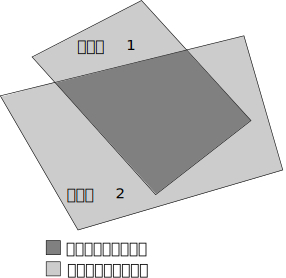
\includegraphics{fig-5-7}
 \caption{重なったパッチのマージ}
 \label{fig:5.7}
\end{figure}


結果的に,スレイブパッチのオリジナルの幾何形状が,
併合の間必ずしも,完全に保存されるというわけではないということです.
したがって,たとえば,円筒状のブロックが,
より大きいブロックにつなげられている場合では,
円筒状の形が正しく保存されるように,
マスタパッチを円筒状のブロックにするのが賢いでしょう.
併合手順を確実に成功させるためのいくつかの追加の推奨策があります.
\begin{itemize}
 \item 2次元の幾何学形状では,2次元平面の外での3次元目のセルサイズは,
       2次元平面でのセルの幅・高さと同様であるべきです.
 \item 二度パッチを併合すること,すなわち,
       \OFkeyword{mergePatchPairs}で二度それを含めるのは勧められません.
 \item 併合されるべきパッチが,他の併合されるパッチと共通の
       辺を共有するところでは,両方がマスタパッチとして宣言されるべきです.
\end{itemize}


\subsection{8頂点未満のブロックの作成}
\label{ssec:5.3.3}
八つ未満の頂点でブロックを作成するために,
1組以上の頂点をお互いの上で潰すことが可能です.
頂点を潰す最も一般的な例としては,
\autoref{ssec:5.2.2}で説明した
\index{wedge@\OFboundary{wedge}!きょうかいじょうけん@境界条件}%
\index{きょうかいじょうけん@境界条件!wedge@\OFboundary{wedge}}%
\OFboundary{wedge}パッチタイプを使用する
2次元の%
\index{じくたいしょう@軸対称!もんだい@問題}%
軸対称問題のための6面のくさび型ブロックを作成するときがあります.
\autoref{fig:5.8}に示す私たちの例における,
ブロックの簡易型のバージョンを使用することで,
過程をわかりやすく例証します.
頂点7を頂点4に,頂点6を頂点5に置いて潰すことによって,
くさび型ブロックを作成したいということです.
これは,ブロック番号7を4で,6を5でそれぞれ交換することによって
簡単にできます.するとブロック番号はこのようになります.
\begin{OFverbatim}[file]
hex (0 1 2 3 4 5 5 4)
\end{OFverbatim}


\begin{figure}[ht]
 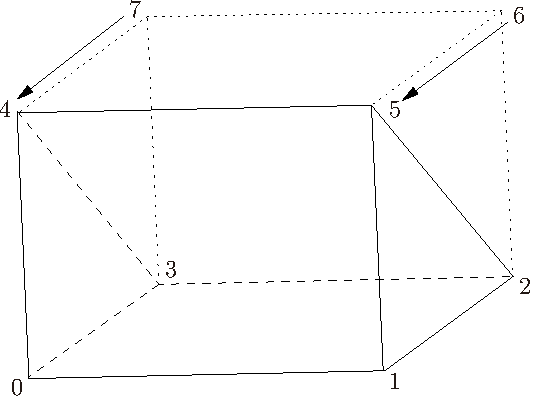
\includegraphics{fig-5-8}
 \caption{くさび形をしたブロックを六つの接点で作る}
 \label{fig:5.8}
\end{figure}


潰れている頂点を含むブロック面を考えることで,
同じことがパッチにも適用でき,以前\OFkeyword{(4 5 6 7)}だったものが,
\OFkeyword{(4 5 5 4)}になります.これは面積をもたないブロック面で,
\OFkeyword{polyMesh}で面のないパッチを生成します.
これは\OFpath{boundary}ファイルにおいて
同様の場合でも見ることができることと同じです.
パッチは\OFdictionary{blockMeshDict}で,
\OFkeyword{empty}として指定されるべきです.
そしてどんなフィールドの境界条件も結果的に\OFkeyword{empty}であるはずです.


\subsection{\OFtool{blockMesh}の実行}
\label{ssec:5.3.4}
\autoref{sec:3.3}で説明されたように,
\OFpath{<case>}ディレクトリのケースに対して
\OFtool{blockMesh}を実行するためには,
以下のようにすればコマンドラインで実行できます.
\begin{OFverbatim}[terminal]
blockMesh -case <case>
\end{OFverbatim}
\index{blockMeshDict@\OFdictionary{blockMeshDict}!ディクショナリ}%
\index{ディクショナリ!blockMeshDict@\OFdictionary{blockMeshDict}}%
\OFdictionary{blockMeshDict}ファイルは,
サブディレクトリ\OFpath{constant/polyMesh}に存在しなければなりません.



\section{\OFtool{snappyHexMesh}ユーティリティを使ったメッシュ生成}
\label{sec:5.4}
\index{snappyHexMesh@\OFtool{snappyHexMesh}!ユーティリティ}%
\index{surface mesh@surface mesh}%
\index{ユーティリティ!snappyHexMesh@\OFtool{snappyHexMesh}}%
\index{メッシュ!せいせい@生成}%
OpenFOAMのメッシュ生成ユーティリティ
\OFtool{snappyHexMesh}について解説します.
\OFtool{snappyHexMesh}は
\index{Stereolithography (STL)}%
STL形式の三角の表面形状から
六面体と
\index{メッシュ!ぶんかつろくめんたい@分割六面体}%
分割六面体の3次元メッシュを自動的に生成します.
初期メッシュから細分化を繰り返し,
できた六面体メッシュを表面に合わせて変形することで,
徐々に表面形状を形成していきます.
オプションとして,できたメッシュを縮小させ,
セルレイヤを挿入することができます.
メッシュの細分化のレベルは非常に柔軟性が高く,
表面の処理はあらかじめ定義したメッシュの水準に適合します.
\OFtool{snappyHexMesh}は毎回負荷を平均化して並列動作をします.


\begin{figure}[ht]
 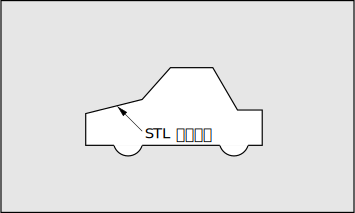
\includegraphics{fig-5-9}
 \caption{\OFtool{snappyHexMesh}における2次元メッシュ問題の概略図}
 \label{fig:5.9}
\end{figure}


\subsection{\OFtool{snappyHexMesh}によるメッシュ生成の過程}
\label{ssec:5.4.1}
\autoref{fig:5.9}に示す概略図を用いて
メッシュを\OFtool{snappyHexMesh}によって生成する流れを説明します.
\index{メッシュ!Stereolithography (STL)}%
Stereolithography (STL) 形式の
\index{メッシュ!ひょうめん@表面}%
表面形状で描かれた対象を囲む長方形の部分
(図中のグレーの部分)にメッシュを作成することを目的とします.
これは外部の空気力学のシミュレーションにおいて典型的な手法です.
あくまでも\OFtool{snappyHexMesh}は3次元メッシュの生成ツールですが,
簡単のためここでは2次元の図を使用しています.

\OFtool{snappyHexMesh}を実行するには以下の準備が必要です.
\begin{itemize}
 \item 2進法またはASCIIで表されたSTL形式による表面形状データを
       ケースディレクトリの\OFpath{constant/triSurface}サブディレクトリに置く.
 \item \autoref{ssec:5.4.2}で述べる\OFtool{blockMesh}を使用して,
       解析領域の範囲とメッシュ密度の基準を決めるために
       六角形の基礎メッシュを作成しておく.
 \item ケースの\OFpath{system}ディレクトリにある
\index{snappyHexMeshDict@\OFpath{snappyHexMeshDict}!ファイル}%
\index{ファイル!snappyHexMeshDict@\OFpath{snappyHexMeshDict}}%
       \OFpath{snappyHexMeshDict}ディクショナリに,適切な内容を入力する.
\end{itemize}
\OFpath{snappyHexMeshDict}ディクショナリには,
\index{snappyHexMesh@\OFtool{snappyHexMesh}!ユーティリティ!メッシュせいせいプロセス@メッシュ生成プロセス}%
メッシュ生成の様々な段階を管理する最上位での変更や,
各過程における個々のサブディレクトリがあります.
入力例を\autoref{tbl:5.7}に示します.


\begin{table}[ht]
 % #! platex UserGuideJa
\begin{tabularx}{\textwidth}{lXl}
 キーワード & 意味 & 例 \\
 \hline
\index{castellatedMesh@\string\OFkeyword{castellatedMesh}!キーワード}%
\index{キーワード!castellatedMesh@\string\OFkeyword{castellatedMesh}}%
 \OFkeyword{castellatedMesh} & 階段状のメッシュを作成するか & \OFkeyword{true} \\
\index{snap@\string\OFkeyword{snap}!キーワード}%
\index{キーワード!snap@\string\OFkeyword{snap}}%
 \OFkeyword{snap} & 表面への適合操作をするか & \OFkeyword{true} \\
\index{doLayers@\string\OFkeyword{doLayers}!キーワード}%
\index{キーワード!doLayers@\string\OFkeyword{doLayers}}%
 \OFkeyword{doLayers} & レイヤの追加をするか & \OFkeyword{true} \\
\index{mergeTolerance@\string\OFkeyword{mergeTolerance}!キーワード}%
\index{キーワード!mergeTolerance@\string\OFkeyword{mergeTolerance}}%
 \OFkeyword{mergeTolerance} &
 マージする許容値.初期メッシュのバウンディングボックスに対する比. &
 \OFkeyword{1e-06} \\
\index{debug@\string\OFkeyword{debug}!キーワード}%
\index{キーワード!debug@\string\OFkeyword{debug}}%
 \OFkeyword{debug} & 中間メッシュと画面出力の制御 \\
 & 最終メッシュのみ出力 & \OFkeyword{0} \\
 & 中間メッシュの出力 & \OFkeyword{1} \\
 & 後処理のため\OFkeyword{cellLevel}を付けた\OFkeyword{volScalarField}を出力 & \OFkeyword{2} \\
 & \OFpath{.obj}ファイルとして中間時の交線を出力 & \OFkeyword{4} \\
\index{geometry@\string\OFkeyword{geometry}!キーワード}%
\index{キーワード!geometry@\string\OFkeyword{geometry}}%
 \OFkeyword{geometry} & 使用する全表面形状のサブディクショナリ \\
\index{castellatedMeshControls@\string\OFkeyword{castellatedMeshControls}!キーワード}%
\index{キーワード!castellatedMeshControls@\string\OFkeyword{castellatedMeshControls}}%
 \OFkeyword{castellatedMeshControls} & 階段状メッシュ制御のサブディクショナリ \\
\index{snapControls@\string\OFkeyword{snapControls}!キーワード}%
\index{キーワード!snapControls@\string\OFkeyword{snapControls}}%
 \OFkeyword{snapControls} & 表面スナップ制御のサブディクショナリ \\
\index{addLayersControls@\string\OFkeyword{addLayersControls}!キーワード}%
\index{キーワード!addLayersControls@\string\OFkeyword{addLayersControls}}%
 \OFkeyword{addLayersControls} & レイヤ追加制御のサブディクショナリ \\
\index{meshQualityControls@\string\OFkeyword{meshQualityControls}!キーワード}%
\index{キーワード!meshQualityControls@\string\OFkeyword{meshQualityControls}}%
 \OFkeyword{meshQualityControls} & メッシュ品質制御のサブディクショナリ \\
 \hline
\end{tabularx}

 \caption{\OFtool{snappyHexMeshDict}の最上位のキーワード}
 \label{tbl:5.7}
\end{table}


\OFtool{snappyHexMesh}で読み込む形状は
\OFpath{snappyHexMeshDict}内の\OFkeyword{geometory}の部分に記述します.
形状は,STLによる表面形状,またはOpenFOAMによる境界形状エントリによって指定できます.

形状はSTL形状またはOpenFOAMにおける幾何実体によって指定されます.
以下に例を示します.
\begin{OFverbatim}[file]
geometry
  {
      sphere.stl // STL filename
      {
          type triSurfaceMesh;
          regions
          {
              secondSolid             // Named region in the STL file
              {
                  name mySecondPatch; // User-defined patch name
              }                       // otherwise given sphere.stl_secondSolid
          }
      }

      box1x1x1  // User defined region name
      {
          type   searchableBox;       // region defined by bounding box
          min    (1.5 1 -0.5);
          max    (3.5 2 0.5);
      }

      sphere2  // User defined region name
      {
          type   searchableSphere;    // region defined by bounding sphere
          centre (1.5 1.5 1.5);
          radius 1.03;
      }
  };
\end{OFverbatim}


\subsection{六面体基礎メッシュの作成}
\label{ssec:5.4.2}
\OFtool{snappyHexMesh}を実行する前に\OFtool{blockMesh}を使用して
\autoref{fig:5.10}が示すように,
解析領域をカバーする六面体セルの
\index{snappyHexMesh@\OFtool{snappyHexMesh}!ユーティリティ!きそメッシュ@基礎メッシュ}%
基礎メッシュを作成します.
基礎メッシュの生成時は以下の点に注意しなければなりません.
\begin{itemize}
 \item メッシュは六面体のみで構成されていること
 \item セルのアスペクト比がほぼ$1$であること.
       少なくとも連続したスナップが行われる表面近傍で
       そうでなければスナップの収束に時間がかかり,不良の原因となる.
 \item STLの表面とセルのエッジが最低でも一箇所は交差すること.
       つまり,一つのセルだけのメッシュでは機能しない.
\end{itemize}


\begin{figure}[ht]
 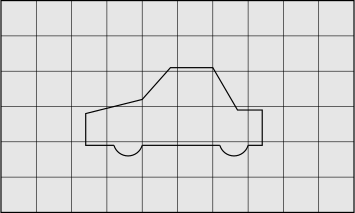
\includegraphics{fig-5-10}
 \caption{\OFtool{snappyHexMesh}実行前の基礎メッシュの生成}
 \label{fig:5.10}
\end{figure}


\subsection{面と輪郭に合わせたセルの分割}
\label{ssec:5.4.3}
\index{snappyHexMesh@\OFtool{snappyHexMesh}!ユーティリティ!セルのぶんかつ@セルの分割}%
セルの分割は,\OFpath{snappyHexMeshDict}の
\index{castellatedMeshControls@\OFsubdictionary{castellatedMeshControls}!ディクショナリ}%
\index{ディクショナリ!castellatedMeshControls@\OFsubdictionary{castellatedMeshControls}}%
\OFsubdictionary{castellatedMeshControls}サブディクショナリにおいて設定して実行します.
\OFsubdictionary{castellatedMeshControls}の入力の例を\autoref{tbl:5.8}に示します.


\begin{table}[ht]
 %#! platex UserGuideJa
\begin{tabularx}{\textwidth}{lXl}
 キーワード & 意味 & 例 \\
 \hline
\index{locationInMesh@\string\OFkeyword{locationInMesh}!キーワード}%
\index{キーワード!locationInMesh@\string\OFkeyword{locationInMesh}}%
 \OFkeyword{locationInMesh} & メッシュが作成される領域内の位置ベクトル & \OFkeyword{(5 0 0)} \\
 & 位置ベクトルが細分化の前または最中にセルの面と一致してはいけない \\
\index{maxLocalCells@\string\OFkeyword{maxLocalCells}!キーワード}%
\index{キーワード!maxLocalCells@\string\OFkeyword{maxLocalCells}}%
 \OFkeyword{maxLocalCells} & 細分化中におけるプロセッサあたりのセルの数の最大値 & \OFkeyword{1e+06} \\
\index{maxGlobalCells@\string\OFkeyword{maxGlobalCells}!キーワード}%
\index{キーワード!maxGlobalCells@\string\OFkeyword{maxGlobalCells}}%
 \OFkeyword{maxGlobalCells} & 細分化中におけるセルの数の総数 (i.e. 除去の前) & \OFkeyword{2e+06} \\
\index{minRefinementCells@\string\OFkeyword{minRefinementCells}!キーワード}%
\index{キーワード!minRefinementCells@\string\OFkeyword{minRefinementCells}}%
 \OFkeyword{minRefinementCells} & 細分化すべきセルの数の最低値.この値以下だと停止 & \OFkeyword{0} \\
\index{nCellsBetweenLevels@\string\OFkeyword{nCellsBetweenLevels}!キーワード}%
\index{キーワード!nCellsBetweenLevels@\string\OFkeyword{nCellsBetweenLevels}}%
 \OFkeyword{nCellsBetweenLevels} & 異なる細分化レベル間のセルの緩衝レイヤーの数 & \OFkeyword{1} \\
\index{resolveFeatureAngle@\string\OFkeyword{resolveFeatureAngle}!キーワード}%
\index{キーワード!resolveFeatureAngle@\string\OFkeyword{resolveFeatureAngle}}%
 \OFkeyword{resolveFeatureAngle} & 角度がこの値を超えている交点をもつセルに最高レベルの細分化を行う & \OFkeyword{30} \\
\index{features@\string\OFkeyword{features}!キーワード}%
\index{キーワード!features@\string\OFkeyword{features}}%
 \OFkeyword{features} & 細分化する特徴辺のリスト \\
\index{refinementSurfaces@\string\OFkeyword{refinementSurfaces}!キーワード}%
\index{キーワード!refinementSurfaces@\string\OFkeyword{refinementSurfaces}}%
 \OFkeyword{refinementSurfaces} & 細分化する表面のディクショナリ \\
\index{refinementRegions@\string\OFkeyword{refinementRegions}!キーワード}%
\index{キーワード!refinementRegions@\string\OFkeyword{refinementRegions}}%
 \OFkeyword{refinementRegions} & 細分化する領域のディクショナリ \\
 \hline
\end{tabularx}

 \caption{\OFdictionary{snappyHexMeshDict}の
\index{castellatedMeshControls@\string\OFsubdictionary{castellatedMeshControls}!ディクショナリ}%
\index{ディクショナリ!castellatedMeshControls@\string\OFsubdictionary{castellatedMeshControls}}%
 \OFsubdictionary{castellatedMeshControls}サブディクショナリのキーワード}
 \label{tbl:5.8}
\end{table}


\begin{figure}[ht]
 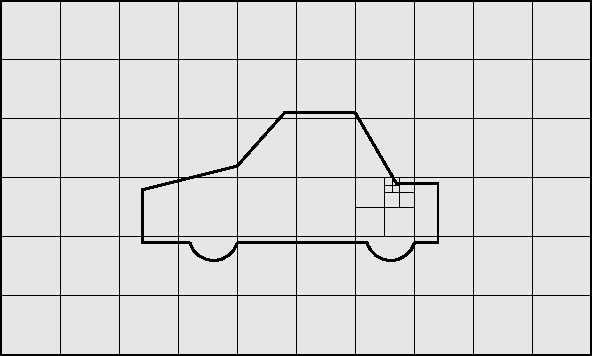
\includegraphics{fig-5-11}
 \caption{\OFtool{snappyHexMesh}メッシングプロセスにおける輪郭によるセル分割}
 \label{fig:5.11}
\end{figure}


分割のプロセスは,\autoref{fig:5.11}に示したように,
まず領域内で指定された輪郭に従って選択されたセルから始まります.
\OFsubdictionary{castellatedMeshControls}サブディクショナリの\OFkeyword{features}リストには,
\OFclass{edgeMesh}のファイル名および細分化の\OFkeyword{level}を含む
ディクショナリ・エントリを記述します.
\begin{OFverbatim}[file]
features
(
    {
        file "features.eMesh"; // file containing edge mesh
        level 2;               // level of refinement
    }
);
\end{OFverbatim}
\OFclass{edgeMesh}に含まれる輪郭データは,
以下のように\OFtool{surfaceFeatureExtract}を使って
\index{surfaceFeatureExtract ユーティリティ@\OFtool{surfaceFeatureExtract} ユーティリティ}%
\index{ユーティリティ!surfaceFeatureExtract@\OFtool{surfaceFeatureExtract}}%
STL形状ファイルから取り出すことができます.
\begin{OFverbatim}[terminal]
surfaceFeatureExtract -includeAngle 150 surface.stl features
\end{OFverbatim}


\begin{figure}[ht]
 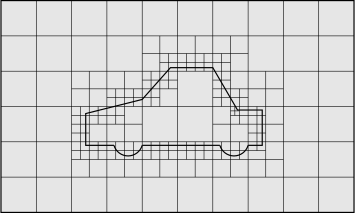
\includegraphics{fig-5-12}
 \caption{\OFtool{snappyHexMesh}メッシングプロセスにおける表面によるセル分割}
 \label{fig:5.12}
\end{figure}


輪郭の細分化に続き,\autoref{fig:5.12}に示すように,
指定された表面における分割のためにセルが選択されます.
\OFkeyword{castellatedMeshControls}の
\OFdictionary{refinementSurface}ディクショナリで,各STL表面のディクショナリ入力と,
型の最小,最大細分化のデフォルトレベルの指定を行います.
(\verb|<min> <max>|) 最小レベルは表面のいたるところに適用され,
最大レベルは
\index{resolveFeatureAngle@\OFkeyword{resolveFeatureAngle}!キーワード}%
\index{キーワード!resolveFeatureAngle@\OFkeyword{resolveFeatureAngle}}%
\OFkeyword{resolveFeatureAngle}に規定される
角度を超過する交点をもつセルに適用されます.

細分化はSTL表面の特定領域に対して複数回行うことができます.
領域の入力は\OFsubdictionary{regions}サブディクショナリに収められています.
各領域の入力に対するキーワードは領域の名前そのものであり,
細分化のレベルはさらにサブのディクショナリに含まれます.以下の入力例を参考にしてください.
\begin{OFverbatim}[file]
refinementSurfaces
  {
      sphere.stl
      {
          level (2 2); // default (min max) refinement for whole surface
          regions
          {
              secondSolid
              {
                  level (3 3); // optional refinement for secondSolid region
              }
          }
      }
  }
\end{OFverbatim}


\subsection{セルの除去}
\label{ssec:5.4.4}
\index{snappyHexMesh@\OFtool{snappyHexMesh}!ユーティリティ!セルのじょきょ@セルの除去}%
輪郭と表面の分割が完了するとセルの除去が始まります.
セルの除去には領域内の有界表面によって完全に囲まれる
一つ以上の範囲が必要です.
セルが保持される領域は,\OFkeyword{castellatedMesh\-Controls}の
\index{locationInMesh@\OFkeyword{locationInMesh}!キーワード}%
\index{キーワード!locationInMesh@\OFkeyword{locationInMesh}}%
\OFkeyword{locationInMesh}キーワードに指定される
領域内の位置ベクトルによって特定されます.
セルの体積のほぼ$50\unit{\%}$以上が領域内に存在する場合保持されます.
残りのセルは\autoref{fig:5.13}に示すように除去されます.


\begin{figure}[ht]
 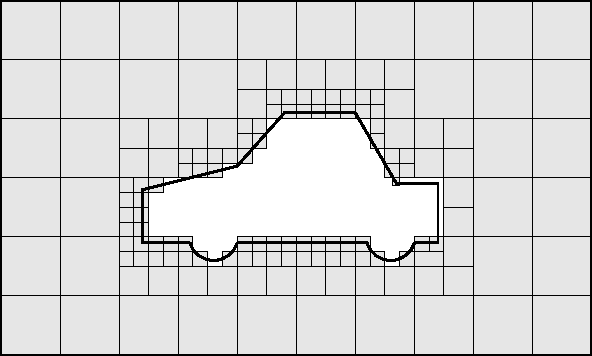
\includegraphics{fig-5-13}
 \caption{\OFtool{snappyHexMesh}メッシングプロセスにおけるセルの除去}
 \label{fig:5.13}
\end{figure}


\subsection{特定領域内のセルの分割}
\label{ssec:5.4.5}
特定領域に含まれるセルはさらに細分化されます.
\autoref{fig:5.14}では長方形の濃いグレーの領域が該当します.
\index{castellatedMeshControls@\OFsubdictionary{castellatedMeshControls}!ディクショナリ}%
\index{ディクショナリ!castellatedMeshControls@\OFsubdictionary{castellatedMeshControls}}%
\OFsubdictionary{castellatedMeshControls}内の
\index{refinementRegions@\OFsubdictionary{refinementRegions}!キーワード}%
\index{キーワード!refinementRegions@\OFsubdictionary{refinementRegions}}%
\OFsubdictionary{refinementRegions}サブディクショナリでは,
\OFsubdictionary{geometry}サブディクショナリにおいて指定された
領域の細分化の入力を行います.細分化の
\index{mode@\OFkeyword{mode}!キーワード}%
\index{キーワード!mode@\OFkeyword{mode}}%
\OFkeyword{mode}と対象領域は以下のとおりです.
\begin{description}
 \item[\OFkeyword{inside}]
\index{inside@\OFkeyword{inside}!キーワードエントリ}%
\index{キーワードエントリ!inside@\OFkeyword{inside}}%
            領域の内部を細分化します.
 \item[\OFkeyword{outside}]
\index{outside@\OFkeyword{outside}!キーワードエントリ}%
\index{キーワードエントリ!outside@\OFkeyword{outside}}%
            領域の外部を細分化します.
 \item[\OFkeyword{distance}]
\index{distance@\OFkeyword{distance}!キーワードエントリ}%
\index{キーワードエントリ!distance@\OFkeyword{distance}}%
            表面からの距離にしたがって細分化します.
            レベルキーワードを用いることで複数の距離にある異なるレベルにも適用できます.
\end{description}
\index{refinementRegions@\OFkeyword{refinementRegions}!キーワード}%
\index{キーワード!refinementRegions@\OFkeyword{refinementRegions}}%
\OFkeyword{refinementRegions}では,細分化のレベルを
\index{levels@\OFkeyword{levels}!キーワード}%
\index{キーワード!levels@\OFkeyword{levels}}%
\OFkeyword{levels}入力リストによって
(\verb|<距離> <レベル>|) のように記述します.
\OFkeyword{inside}と\OFkeyword{outside}の細分化の場合,
\verb|<distance>|は不要で無視されますが,
指定する必要があります.以下に入力例を示します.
\begin{OFverbatim}[file]
refinementRegions
{
    box1x1x1
    {
        mode inside;
        levels ((1.0 4));         // refinement level 4 (1.0 entry ignored)
    }

    sphere.stl
    {                             // refinement level 5 within 1.0 m
        mode distance;            // refinement level 3 within 2.0 m
        levels ((1.0 5) (2.0 3)); // levels must be ordered nearest first
    }
}
\end{OFverbatim}


\begin{figure}[ht]
 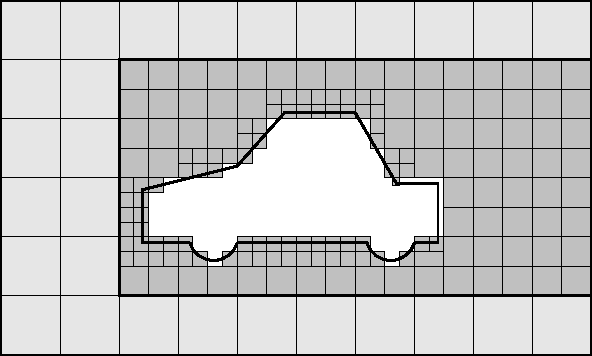
\includegraphics{fig-5-14}
 \caption{\OFtool{snappyHexMesh}メッシングプロセスにおける領域によるセル分割}
 \label{fig:5.14}
\end{figure}


\subsection{面へのスナップ}
\label{ssec:5.4.6}
\index{snappyHexMesh@\OFtool{snappyHexMesh}!ユーティリティ!めんへのスナップ@面へのスナップ}%
メッシュを生成する次の段階として,
メッシュを平滑化するためにセルの頂点を表面に移動します.
その手順は以下の通りです.
\begin{enumerate}
 \item\label{enm:5.4.6-1}
      ギザギザの境界面の頂点をSTL表面上に移動する
 \item\label{enm:5.4.6-2}
      最後に移動した境界の頂点を用いて内部メッシュの緩和を求める
 \item メッシュの水準に影響をもたらす頂点を探す
 \item 最初の数値 (\ref{enm:5.4.6-1}) での頂点の移動を減らし,
       \ref{enm:5.4.6-2}からメッシュの質が
       満足できるレベルに達するまで繰り返す.
\end{enumerate}
\autoref{tbl:5.9}に示す\OFpath{snappyHexMeshDict}の
\OFsubdictionary{snapControls}サブディクショナリにおいて設定をします.


\begin{table}[ht]
 %#! platex UserGuideJa
\begin{tabularx}{\textwidth}{lXl}
 キーワード & 意味 & 例 \\
 \hline
\index{nSmoothPatch@\string\OFkeyword{nSmoothPatch}!キーワード}%
\index{キーワード!nSmoothPatch@\string\OFkeyword{nSmoothPatch}}%
 \OFkeyword{nSmoothPatch} & 表面との一致に至る前に行うパッチの平滑化の回数 & 3 \\
\index{tolerance@\string\OFkeyword{tolerance}!キーワード}%
\index{キーワード!tolerance@\string\OFkeyword{tolerance}}%
 \OFkeyword{tolerance} & 局所的な輪郭の最大長さに対する点と表面の距離の比の許容範囲 & 4.0 \\
\index{nSolveIter@\string\OFkeyword{nSolveIter}!キーワード}%
\index{キーワード!nSolveIter@\string\OFkeyword{nSolveIter}}%
 \OFkeyword{nSolveIter} & メッシュの置き換え時の緩和計算の回数 & 30 \\
\index{nRelaxIter@\string\OFkeyword{nRelaxIter}!キーワード}%
\index{キーワード!nRelaxIter@\string\OFkeyword{nRelaxIter}}%
 \OFkeyword{nRelaxIter} & メッシュのスナップ時の緩和計算の最大回数 & 5 \\
 \hline
\end{tabularx}

 \caption{\OFkeyword{snapControls}のキーワード}
 \label{tbl:5.9}
\end{table}


\autoref{fig:5.15}に概略図に例を示します.
(メッシュの動きは多少現実と異なるように見えています.)


\begin{figure}[ht]
 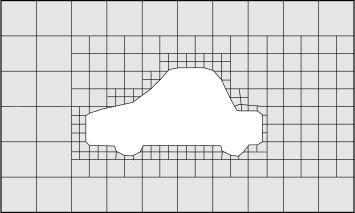
\includegraphics{fig-5-15}
 \caption{\OFtool{snappyHexMesh}メッシングプロセスにおける表面のスナップ}
 \label{fig:5.15}
\end{figure}


\subsection{メッシュレイヤ}
\label{ssec:5.4.7}
\index{snappyHexMesh@\OFtool{snappyHexMesh}!ユーティリティ!メッシュレイヤ}%
境界面に沿った不規則なセルを作りもしますが,
スナップによるメッシュの生成は目的に合致するでしょう.
メッシュをかける過程にはさらにオプションがあり,
\autoref{fig:5.16}の暗く影のついた部分が示すように,
境界面に沿って並べられた六面体のセルのレイヤを追加します.


\begin{figure}[ht]
 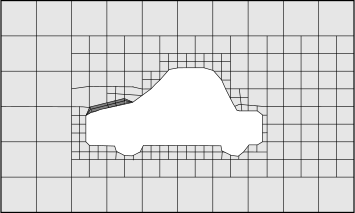
\includegraphics{fig-5-16}
 \caption{\OFtool{snappyHexMesh}メッシングプロセスにおけるレイヤの挿入}
 \label{fig:5.16}
\end{figure}


メッシュのレイヤの追加は,
以下の手順のように既存のメッシュを境界から縮小させ,
レイヤを挿入することで行われます.
\begin{enumerate}
 \item 表面に対して法線方向の厚み分だけメッシュを投影させる.
 \item\label{enm:5.4.7-2}
      最後に移動した境界面の頂点をもとに内部メッシュの緩和を計算する
 \item 有効性を確認し,満足されていない場合は投影された厚みを減らし,
       \ref{enm:5.4.7-2}からやり直す.
       いかなる厚みでも有効性が満足できない場合はレイヤを挿入しない.
 \item 有効性が確認できたらレイヤメッシュを挿入する.
 \item メッシュを再度チェックし,不良箇所が見られる場合は
       レイヤを除去し\ref{enm:5.4.7-2}に戻る.
\end{enumerate}

レイヤの追加の手順は\OFdictionary{snappyHexMeshDict}の
\OFsubdictionary{addLayersControls}サブディクショナリの設定によって行われます.
入力されるものは\autoref{tbl:5.10}に示すとおりです.


\begin{table}[ht]
 %#! platex UserGuideJa
\begin{tabularx}{\textwidth}{lXl}
 キーワード & 意味 & 例 \\
 \hline
\index{layers@\string\OFkeyword{layers}!キーワード}%
\index{キーワード!layers@\string\OFkeyword{layers}}%
 \OFkeyword{layers} &
     レイヤのディクショナリ &
          \\
\index{relativeSizes@\string\OFkeyword{relativeSizes}!キーワード}%
\index{キーワード!relativeSizes@\string\OFkeyword{relativeSizes}}%
 \OFkeyword{relativeSizes} &
     レイヤ厚さを,レイヤ外部の歪んでいないセルの大きさに対する相対値とするか,
     または絶対値とするか &
         \OFkeyword{true}/\OFkeyword{false} \\
\index{expansionRatio@\string\OFkeyword{expansionRatio}!キーワード}%
\index{キーワード!expansionRatio@\string\OFkeyword{expansionRatio}}%
 \OFkeyword{expansionRatio} &
     レイヤメッシュの拡大比率 &
         \OFkeyword{1.0} \\
\index{finalLayerRatio@\string\OFkeyword{finalLayerRatio}!キーワード}%
\index{キーワード!finalLayerRatio@\string\OFkeyword{finalLayerRatio}}%
 \OFkeyword{finalLayerRatio} &
     壁から最も遠い層の厚さ.
     \OFkeyword{relativeSizes}エントリにより相対値か絶対値かが決まる &
         \OFkeyword{0.3} \\
\index{minThickness@\string\OFkeyword{minThickness}!キーワード}%
\index{キーワード!minThickness@\string\OFkeyword{minThickness}}%
 \OFkeyword{minThickness} &
     セルのレイヤの最小の厚さ.
     相対値または絶対値(同上) &
         \OFkeyword{0.25} \\
\index{nGrow@\string\OFkeyword{nGrow}!キーワード}%
\index{キーワード!nGrow@\string\OFkeyword{nGrow}}%
 \OFkeyword{nGrow} &
     点を押し出さないと生成されない面に結合されたレイヤの数.
     輪郭に近いレイヤ追加の収束に役立つ. &
         \OFkeyword{1} \\
\index{featureAngle@\string\OFkeyword{featureAngle}!キーワード}%
\index{キーワード!featureAngle@\string\OFkeyword{featureAngle}}%
 \OFkeyword{featureAngle} &
     この角度以上では表面は押し出されない &
         \OFkeyword{60} \\
\index{nRelaxIter@\string\OFkeyword{nRelaxIter}!キーワード}%
\index{キーワード!nRelaxIter@\string\OFkeyword{nRelaxIter}}%
 \OFkeyword{nRelaxIter} &
     スナップの緩和反復の最大回数 &
         \OFkeyword{5} \\
\index{nSmoothSurfaceNormals@\string\OFkeyword{nSmoothSurfaceNormals}!キーワード}%
\index{キーワード!nSmoothSurfaceNormals@\string\OFkeyword{nSmoothSurfaceNormals}}%
 \OFkeyword{nSmoothSurfaceNormals} &
     表面法線のスムージング反復数 &
         \OFkeyword{1} \\
\index{nSmoothNormals@\string\OFkeyword{nSmoothNormals}!キーワード}%
\index{キーワード!nSmoothNormals@\string\OFkeyword{nSmoothNormals}}%
 \OFkeyword{nSmoothNormals} &
     内部メッシュの運動方向のスムージング反復数 &
         \OFkeyword{3} \\
\index{nSmoothThickness@\string\OFkeyword{nSmoothThickness}!キーワード}%
\index{キーワード!nSmoothThickness@\string\OFkeyword{nSmoothThickness}}%
 \OFkeyword{nSmoothThickness} &
     表面パッチ上の滑らかなレイヤの厚さ &
         \OFkeyword{10} \\
\index{maxFaceThicknessRatio@\string\OFkeyword{maxFaceThicknessRatio}!キーワード}%
\index{キーワード!maxFaceThicknessRatio@\string\OFkeyword{maxFaceThicknessRatio}}%
 \OFkeyword{maxFaceThicknessRatio} &
     極端にゆがんでいるセルでレイヤの生成を止める &
         \OFkeyword{0.5} \\
\index{maxThicknessToMedialRatio@\string\OFkeyword{maxThicknessToMedialRatio}!キーワード}%
\index{キーワード!maxThicknessToMedialRatio@\string\OFkeyword{maxThicknessToMedialRatio}}%
 \OFkeyword{maxThicknessToMedialRatio} &
     中間の距離と厚さの比が大きくなるとレイヤの生成を抑制する &
         \OFkeyword{0.3} \\
\index{minMedianAxisAngle@\string\OFkeyword{minMedianAxisAngle}!キーワード}%
\index{キーワード!minMedianAxisAngle@\string\OFkeyword{minMedianAxisAngle}}%
 \OFkeyword{minMedianAxisAngle} &
     中間の軸点選択に使う角度 &
         \OFkeyword{130} \\
\index{nBufferCellsNoExtrude@\string\OFkeyword{nBufferCellsNoExtrude}!キーワード}%
\index{キーワード!nBufferCellsNoExtrude@\string\OFkeyword{nBufferCellsNoExtrude}}%
 \OFkeyword{nBufferCellsNoExtrude} &
     新しいレイヤの末端のためのバッファ領域を作成 &
         \OFkeyword{0} \\
\index{nLayerIter@\string\OFkeyword{nLayerIter}!キーワード}%
\index{キーワード!nLayerIter@\string\OFkeyword{nLayerIter}}%
 \OFkeyword{nLayerIter} &
     レイヤを追加する反復計算全体の最大反復数 &
         \OFkeyword{50} \\
\index{nRelaxedIter@\string\OFkeyword{nRelaxedIter}!キーワード}%
\index{キーワード!nRelaxedIter@\string\OFkeyword{nRelaxedIter}}%
 \OFkeyword{nRelaxedIter} &
     この反復回数を超えた後は,\OFkeyword{meshQuality}の
     \OFsubdictionary{relaxed}サブディクショナリにおける制御値が使われる &
         \OFkeyword{20} \\
 \hline
\end{tabularx}

 \caption{\OFpath{snappyHexMeshDict}の\OFsubdictionary{addLayersControls}サブディクショナリのキーワード}
 \label{tbl:5.10}
\end{table}


レイヤのサブディクショナリはレイヤが適用される各パッチと
必要な表面レイヤの数の入力を含んでいます.
レイヤ追加は表面形状ではなく,できあがったメッシュに関連しているのでパッチ名が使われ,
したがって表面領域に対してではなくパッチに対して適用されます.
レイヤの入力例は以下のとおりです.
\begin{OFverbatim}[file]
 layers
  {
      sphere.stl_firstSolid
      {
          nSurfaceLayers 1;
      }
      maxY
      {
          nSurfaceLayers 1;
      }
  }
\end{OFverbatim}


\begin{table}[ht]
 %#! platex UserGuideJa
\begin{tabularx}{\textwidth}{lXl}
 キーワード & 意味 & 例 \\
 \hline
\index{maxNonOrtho@\OFkeyword{maxNonOrtho}!キーワード}%
\index{キーワード!maxNonOrtho@\OFkeyword{maxNonOrtho}}%
 \OFkeyword{maxNonOrtho} &
     非直交性上限角.\OFkeyword{180}は不可 &
         \OFkeyword{65} \\
\index{maxBoundarySkewness@\OFkeyword{maxBoundarySkewness}!キーワード}%
\index{キーワード!maxBoundarySkewness@\OFkeyword{maxBoundarySkewness}}%
 \OFkeyword{maxBoundarySkewness} &
     境界面ひずみ上限値.${} < 0$は不可 &
         \OFkeyword{20} \\
\index{maxInternalSkewness@\OFkeyword{maxInternalSkewness}!キーワード}%
\index{キーワード!maxInternalSkewness@\OFkeyword{maxInternalSkewness}}%
 \OFkeyword{maxInternalSkewness} &
     内部面ひずみ上限値.${} < 0$は不可 &
         \OFkeyword{4} \\
\index{maxConcave@\OFkeyword{maxConcave}!キーワード}%
\index{キーワード!maxConcave@\OFkeyword{maxConcave}}%
 \OFkeyword{maxConcave} &
     凹み上限角.\OFkeyword{180}は不可 &
         \OFkeyword{80} \\
\index{minFlatness@\OFkeyword{minFlatness}!キーワード}%
\index{キーワード!minFlatness@\OFkeyword{minFlatness}}%
 \OFkeyword{minFlatness} &
     実際の領域に対する最小の投影面積比率.\OFkeyword{-1}は不可 &
         \OFkeyword{0.5} \\
\index{minVol@\OFkeyword{minVol}!キーワード}%
\index{キーワード!minVol@\OFkeyword{minVol}}%
 \OFkeyword{minVol} &
     最小のピラミッドボリューム.大きな絶対値の負の数(例えば\OFkeyword{-1e30})は不可 &
         \OFkeyword{1e-13} \\
\index{minArea@\OFkeyword{minArea}!キーワード}%
\index{キーワード!minArea@\OFkeyword{minArea}}%
 \OFkeyword{minArea} &
     最小面領域.${} < 0$は不可 &
         \OFkeyword{} \\
\index{minTwist@\OFkeyword{minTwist}!キーワード}%
\index{キーワード!minTwist@\OFkeyword{minTwist}}%
 \OFkeyword{minTwist} &
     最小面ねじれ.${} < -1$は不可 &
         \OFkeyword{0.05} \\
\index{minDeterminant@\OFkeyword{minDeterminant}!キーワード}%
\index{キーワード!minDeterminant@\OFkeyword{minDeterminant}}%
 \OFkeyword{minDeterminant} &
     最小正常セルの行列式.$\mbox{\OFkeyword{1}} = \mbox{\OFkeyword{hex}}$,${} \le 0$は不法なセル &
         \OFkeyword{0.001} \\
\index{minFaceWeight@\OFkeyword{minFaceWeight}!キーワード}%
\index{キーワード!minFaceWeight@\OFkeyword{minFaceWeight}}%
 \OFkeyword{minFaceWeight} &
     $\mbox{\OFkeyword{0}} \rightarrow \mbox{\OFkeyword{0.5}}$ &
         \OFkeyword{0.05} \\
\index{minVolRatio@\OFkeyword{minVolRatio}!キーワード}%
\index{キーワード!minVolRatio@\OFkeyword{minVolRatio}}%
 \OFkeyword{minVolRatio} &
     $\mbox{\OFkeyword{0}} \rightarrow \mbox{\OFkeyword{1.0}}$ &
         \OFkeyword{0.01} \\
\index{minTriangleTwist@\OFkeyword{minTriangleTwist}!キーワード}%
\index{キーワード!minTriangleTwist@\OFkeyword{minTriangleTwist}}%
 \OFkeyword{minTriangleTwist} &
     Fluent計算可能性では${} > 0$ & \\
\index{nSmoothScale@\OFkeyword{nSmoothScale}!キーワード}%
\index{キーワード!nSmoothScale@\OFkeyword{nSmoothScale}}%
 \OFkeyword{nSmoothScale} &
     エラー分布反復数 &
         \OFkeyword{4} \\
\index{errorReduction@\OFkeyword{errorReduction}!キーワード}%
\index{キーワード!errorReduction@\OFkeyword{errorReduction}}%
 \OFkeyword{errorReduction} &
     エラー点の置換のための減少量 &
         \OFkeyword{} \\
\index{relaxed@\OFkeyword{relaxed}!キーワード}%
\index{キーワード!relaxed@\OFkeyword{relaxed}}%
 \OFkeyword{relaxed} &
     上述の各キーワードエントリに対して,
     レイヤ追加プロセス中に反復回数が\OFkeyword{nRelaxedIter}を
     超えたときに使われる修正値を含んだサブディクショナリ
      &
         \parbox[t]{4em}{\ttfamily relaxed\par\{\par\ldots\par\}} \\
 \hline
\end{tabularx}

 \caption{\OFdictionary{snappyHexMeshDict}の
 \OFsubdictionary{meshQualityControls}サブディクショナリのキーワード}
 \label{tbl:5.11}
\end{table}


\subsection{メッシュの品質制御}
\label{ssec:5.4.8}
メッシュの品質は\OFdictionary{snappyHexMeshDict}の
\OFsubdictionary{meshQualityControls}サブディクショナリへ入力することで
制御できます.入力は\autoref{tbl:5.11}に示します.



\section{メッシュの変換}
\label{sec:5.5}
ユーザは,他のパッケージを使用してメッシュを生成し,
OpenFOAMが用いる形式にそれらを変換できます.
\autoref{tbl:3.6}に示したような
様々なメッシュ変換ユーティリティが用意されています.

よく使われるメッシュ変換ユーティリティのいくつかを以下に挙げ,
使い方を紹介します.
\begin{description}
 \item[\OFtool{fluentMeshToFoam}]
\index{fluentMeshToFoam@\OFtool{fluentMeshToFoam}!ユーティリティ}%
\index{ユーティリティ!fluentMeshToFoam@\OFtool{fluentMeshToFoam}}%
            \OFemph{Fluent}の\texttt{.msh}メッシュファイルを読み込みます.
            2次元,3次元両方に使えます.
 \item[\OFtool{starToFoam}]
\index{starToFoam@\OFtool{starToFoam}!ユーティリティ}%
\index{ユーティリティ!starToFoam@\OFtool{starToFoam}}%
            \OFemph{STAR-CD}/\OFemph{PROSTAR}のメッシュファイルを読み込みます.
 \item[\OFtool{gambitToFoam}]
\index{gambitToFoam@\OFtool{gambitToFoam}!ユーティリティ}%
\index{ユーティリティ!gambitToFoam@\OFtool{gambitToFoam}}%
            \OFemph{GAMBIT}の\texttt{.neu}ニュートラルファイルを読み込みます.
 \item[\OFtool{ideasToFoam}]
\index{ideasToFoam@\OFtool{ideasToFoam}!ユーティリティ}%
\index{ユーティリティ!ideasToFoam@\OFtool{ideasToFoam}}%
            \OFemph{ANSYS}の\texttt{.ans}形式で書かれた
            \OFemph{I-DEAS}メッシュを読み込みます.
 \item[\OFtool{cfx4ToFoam}]
\index{cfx4ToFoam@\OFtool{cfx4ToFoam}!ユーティリティ}%
\index{ユーティリティ!cfx4ToFoam@\OFtool{cfx4ToFoam}}%
            \texttt{.geo}形式で書かれた\OFemph{CFX}メッシュを読み込みます.
\end{description}


\subsection{\OFtool{fluentMeshToFoam}}
\label{ssec:5.5.1}
Fluentは,\texttt{.msh}拡張子をもつ単一のファイルに,
メッシュ・データを書き出します.
ASCII書式でファイルを書かなければなりませんが,
それは,Fluentのデフォルト設定ではありません.
2次元の幾何形状を含んでいる単一の流れの
Fluentメッシュを変換することは可能です.
OpenFOAMでは,2次元幾何形状は,現在のところ,
3次元でメッシュを定義することで扱われます.
そこでは,前面と背面は\OFkeyword{empty}境界パッチタイプと定義されます.
2次元のFluentメッシュを読みこむときに,
コンバータは,自動的に3次元目の方向にメッシュを拡張し,
\OFkeyword{frontAndBackPlanes}と名づけ,空のパッチを加えます.

また,以下の特徴が見られます.
\begin{itemize}
 \item OpenFOAMコンバータは,
       Fluentの境界条件の定義をできるだけ把握しようと試みるでしょう.
       しかしながら,OpenFOAMとFluentの境界条件の間に明確で,
       直接的な対応は全くないので,
       ユーザはケースを実行する前に境界条件をチェックするべきです.
 \item 2次元メッシュから軸対称なメッシュを生成することは
       現在サポートされていませんが,需要があれば実装されるでしょう.
 \item 複数の媒質からなるメッシュは受入れられません.
       もし複数の流体媒質が存在していると,
       それらは単一のOpenFOAMメッシュに変換されます.
       もし固体領域が検出されると,
       コンバータは,それを排除しようと試みます.
 \item Fluentではメッシュの内部にパッチを定義することができます.
       つまり,面の両側にセルが存在する場合です.
       そのようなパッチはOpenFOAMでは許容されていないので,
       コンバータはそれらを排除しようと試みます.
 \item 現在,埋め込まれたインタフェースと
       細分化ツリーに関してはサポートされていません.
\end{itemize}
Fluent \texttt{.msh}ファイルの変換手順は,
まず必要なディレクトリとファイルを作成して
新しいOpenFOAMケースを作ることから始めます.
ケースディレクトリには,\OFpath{system}サブディレクトリの中に
\OFdictionary{controlDict}ファイルをおきます.
そして以下のコマンドを実行します.
\begin{OFverbatim}[terminal]
fluentMeshToFoam <meshFile>
\end{OFverbatim}
ここで \texttt{<meshFile>} は絶対パスか相対パスによる
\texttt{.msh}ファイルの名前です.


\subsection{\OFtool{starToFoam}}
\label{ssec:5.5.2}
本節ではSTAR-CDコードで生成されたメッシュを,
OpenFOAMのメッシュのクラスが読むことができる形式に変換する方法を説明します.
メッシュはSTAR-CDとともに供給されるどのパッケージでも生成できます.
例えばPROSTAR,SAMM,ProAMおよびそれらの派生物です.
コンバータは,統合された任意のカップルマッチングを含む
どんな単一流れのメッシュも受け入れ,
すべてのセルタイプがサポートされます.
コンバータがサポートしない特徴は以下のとおりです.
\begin{itemize}
 \item 複数の流れのメッシュの仕様
 \item バッフル,すなわち,領域内に挿入された厚さなしの壁
 \item 部分境界,カップルマッチのうちの
       覆われていない部分は境界面であると考えられます.
 \item スライディング・インタフェース
\end{itemize}
複数の流れを含むメッシュに関しては,
それぞれの独立した流れを別々のメッシュとして書き出し,
それらをOpenFOAMで組み立て直すことで,メッシュ変換が実現できます.

OpenFOAMは,\autoref{sec:5.1}で指定された
かなり厳しい妥当性評価基準に整合しているメッシュの入力だけを
受け入れるという方針を採ります.
無効なメッシュを用いて実行されることはなく,
それ自体が無効なメッシュは変換できません.
以下の節では,STAR-CDとともに供給された
メッシュ生成パッケージを用いてメッシュを生成する際に,
OpenFOAM形式に変換できることを保証するために
取らなければならない方法を説明します.
これからの節において重複を避けるために,
STAR-CDとともに供給されるメッシュ生成ツールは,
STAR-CDという総称によって参照されることにします.

\subsubsection{変換における一般的なアドバイス}
\label{sssec:5.5.2.1}
\OFtool{starToFoam}の変換を試みる前に,
STAR-CDのメッシュチェックツールを実行することをお勧めします.
そして変換の後に,新たに変換されたメッシュで
\index{checkMesh@\OFtool{checkMesh}!ユーティリティ}%
\index{ユーティリティ!checkMesh@\OFtool{checkMesh}}%
\OFtool{checkMesh}ユーティリティを実行するべきです.
あるいは,\OFtool{starToFoam}は,ユーザが問題のあるセルに
注目することができるように,
\textsf{PROSTAR}コマンドを含む警告を出すことがあります.
問題の多いセルとマッチは,OpenFOAMでメッシュを使おうとする前に
チェックして修正するべきです.
OpenFOAMで動作しない無効なメッシュでも,
課される妥当性評価基準が異なる別の環境では
動くかもしれないことを覚えておいてください.

許容誤差のマッチングに関するいくつかの問題は,
コンバータのマッチング許容誤差を使って解決することができます.
しかしながら,その有効性には限界があり,
マッチング許容誤差をデフォルトレベルから増加させることが
明らかに必要であるということは,
オリジナルのメッシュが正確でないことを示します.

\subsubsection{不要なデータの消去}
\label{sssec:5.5.2.2}
メッシュ生成が終了したら,流体セルが作成されて,
他のすべてのセルが取り除かれると仮定して,
あらゆる不要な頂点を取り除き,
セル境界と頂点番号を圧縮してください.
これは以下の\textsf{PROSTAR}コマンドで実行されます.
\begin{OFverbatim}[terminal]
CSET NEWS FLUID
CSET INVE
\end{OFverbatim}
\texttt{CSET}は空であるべきです.そうでないなら,
\texttt{CSET}でセルを調べて,モデルを調整してください.
もしセルを本当に必要としていないなら,
\textsf{PROSTAR}コマンドを使用することでそれらを取り除くことができます.
\begin{OFverbatim}[terminal]
CDEL CSET
\end{OFverbatim}
同様に,頂点も取り除く必要があるでしょう.
\begin{OFverbatim}[terminal]
CSET NEWS FLUID
VSET NEWS CSET
VSET INVE
\end{OFverbatim}
これらの必要でない頂点を取り除く前に,
不要な境界面を集めておかなければなりません.
\begin{OFverbatim}[terminal]
CSET NEWS FLUID
VSET NEWS CSET
BSET NEWS VSET ALL
BSET INVE
\end{OFverbatim}
\texttt{BSET}が空でないなら,不要な境界面は
以下のコマンドを使用して削除することができます.
\begin{OFverbatim}[terminal]
BDEL BSET
\end{OFverbatim}
このとき,モデルは定義された境界面と同様に,
流体セルとそれを支持する頂点だけを含むべきです.
すべての境界面はセルの頂点によって完全に支えられるべきです.
もしそうでないなら,すべてが正常になるまで幾何学形状を正常化し続けます.

\subsubsection{デフォルトの境界条件の削除}
\label{sssec:5.5.2.3}
デフォルトでSTAR-CDは,明示的に境界領域と結びつけられていない
全ての境界面に対して壁境界を適用します.
そのほかの境界面は,\texttt{default}境界領域に集められ,
境界タイプ\texttt{0}として割り当てられます.
これは人為ミスを誘発するので,OpenFOAMは,
未定義の界面のための\texttt{default}境界条件の概念を意図的に用意していません.
例えば,すべての未定義の境界面にデフォルト条件を
意図して与えたかどうかをチェックする手段は全くありません.

したがって,メッシュが首尾よく変換されるために,
各OpenFOAMメッシュに対するすべての境界を指定しなければなりません.
以下で説明された手順を用いることで
\texttt{default}境界を実際の境界条件に変更する必要があります.
\begin{enumerate}
 \item \OFkeyword{Wire Surface}オプションで幾何形状をプロットしてください.
 \item \OFkeyword{default}領域0と同じパラメータで
       追加の境界領域を定義してください.
       そして,境界ツールでゾーン指定を選択し,
       スクリーンに描かれたモデル全体のまわりに多角形を描くことで,
       全ての見えている面を10などの新しい領域に加えてください.
       \textsf{PROSTAR}で以下のコマンドを実行することによって,
       これができます.
\begin{OFverbatim}[terminal]
RDEF 10 WALL
BZON 10 ALL
\end{OFverbatim}
 \item そのセットから,すでに定義されている境界タイプを全て外してください.
       境界領域から実行していきます.
\begin{OFverbatim}[terminal]
BSET NEWS REGI 1
BSET NEWS REGI 2
... 3, 4, ...
\end{OFverbatim}
       境界セットに関連している頂点を集め,
       次に頂点に関連している境界面を集めてください.
       それらは元のセットのように$2$倍あるでしょう.
\begin{OFverbatim}[terminal]
BSET NEWS REGI 1
VSET NEWS BSET
BSET NEWS VSET ALL
BSET DELE REGI 1
REPL
\end{OFverbatim}
       これは境界領域1の上で定義された境界領域10の面を与えるはずです.
       \verb|BDEL BSET|と入力して,それらを削除してください.
       すべての領域にこれらを繰り返してください.
\end{enumerate}

\subsubsection{モデルの再番号付け}
\label{sssec:5.5.2.4}
コマンドを使用することでモデルの番号を付け替えて,チェックしてください.
\begin{OFverbatim}[terminal]
CSET NEW FLUID
CCOM CSET
VSET NEWS CSET
VSET INVE (Should be empty!)
VSET INVE
VCOM VSET
BSET NEWS VSET ALL
BSET INVE (Should be empty also!)
BSET INVE
BCOM BSET
CHECK ALL
GEOM
\end{OFverbatim}
内部の\textsf{PROSTAR}の照合は,最後の二つのコマンドで実行されます.
コマンドはいくつかの予見できない誤りを明らかにするかもしれません.
また,\textsf{PROSTAR}は幾何学形状にではなく,
STAR-CDのために因子を適用するだけであるので,
スケール因子に注意してください.因子が1でないなら,
OpenFOAMの
\index{scalePoints@\OFtool{scalePoints}!ユーティリティ}%
\index{ユーティリティ!scalePoints@\OFtool{scalePoints}}%
\OFtool{scalePoints}ユーティリティを使用してください.

\subsubsection{メッシュデータの出力}
\label{sssec:5.5.2.5}
メッシュがいったん完成されたら,
モデルのすべての統合されたマッチをカップルタイプ1に置いてください.
他のすべてのタイプが,任意のマッチを示すのに使用されるでしょう.
\begin{OFverbatim}[terminal]
CPSET NEWS TYPE INTEGRAL
CPMOD CPSET 1
\end{OFverbatim}
そして,計算格子の構成要素をそれら自身のファイルに書かなければなりません.
これは以下のコマンドを実行し,境界に対して\textsf{PROSTAR}を用いることで行います.
\begin{OFverbatim}[terminal]
BWRITE
\end{OFverbatim}
デフォルトでは,これは\texttt{.23}ファイル(3.0の前のバージョン)か
\texttt{.bnd}ファイル(バージョン3.0以降)に書きます.
セルに対しては,以下のコマンド,
\begin{OFverbatim}[terminal]
CWRITE
\end{OFverbatim}
がセルを\texttt{.14}か\texttt{.cel}ファイルに出力します.
頂点に対しては,以下のコマンド,
\begin{OFverbatim}[terminal]
VWRITE
\end{OFverbatim}
が\texttt{.15}か\texttt{.vrt}ファイルに出力します.
現在の既定の設定では,ASCII書式でファイルを書き出します.
カップルが存在しているなら,
拡張子\texttt{.cpl}をもつ追加カップルファイルが
以下のコマンドをタイプすることによって書きだす必要があります.
\begin{OFverbatim}[terminal]
CPWRITE
\end{OFverbatim}
三つのファイルに出力した後に,\textsf{PROSTAR}を終了するか,
ファイルを閉じてください.
パネルに目を通して,すべてのSTAR-CDのサブモデル,
材料,および流体の特性に注目してください.
材料の特性と数学的モデルは,OpenFOAMディクショナリファイルを作成し,
編集することで設定する必要があります.

\textsf{PROSTAR}ファイルを変換する手順は最初に,
必要なディレクトリを作成することで新しいOpenFOAMのケースを作ることです.
同じディレクトリの中に\textsf{PROSTAR}ファイルを格納しなければなりません.
そして,ユーザはファイル拡張子を変えなければなりません.
\texttt{.23}と\texttt{.14}と\texttt{.15} (STAR-CDバージョン3.0以前) か,
\texttt{.pcs}と\texttt{.cls}と\texttt{.vtx} (STAR-CDバージョン3.0以降) から,
それぞれ\texttt{.bnd},\texttt{.cel},および\texttt{.vrt}に変えます.

\subsubsection{\texttt{.vrt}ファイルの問題}
\label{sssec:5.5.2.6}
\texttt{.vrt}ファイルは,フリー・フォーマットというよりむしろ
指定された幅に関するデータ列で書かれています.
座標値が続く頂点番号を与えるデータの典型的な行は,
以下のとおりです.
\begin{OFverbatim}[file]
19422 -0.105988957 -0.413711881E-02 0.000000000E+00
\end{OFverbatim}
縦座標が科学表記法で書かれていて,
負であるなら,値の間には,スペースが全くないこともあります.
例えば以下のような状況です.
\begin{OFverbatim}[file]
19423 -0.953953117E-01-0.338810333E-02 0.000000000E+00
\end{OFverbatim}
\OFtool{starToFoam}コンバータは,
縦座標の値を区切るためにスペースを区切り文字としてデータを読むので,
前の例を読むとき,問題になります.
したがって,OpenFOAMは必要なところで値の間にスペースを挿入するための
簡単なスクリプト,
\index{foamCorrectVrt@\OFtool{foamCorrectVrt}!スクリプト/エイリアス}%
\index{スクリプト/エイリアス!foamCorrectVrt@\OFtool{foamCorrectVrt}}%
\OFtool{foamCorrectVrt}を含んでいます.
すると,それが前の例を以下のように変換するでしょう.
\begin{OFverbatim}[file]
19423 -0.953953117E-01 -0.338810333E-02 0.000000000E+00
\end{OFverbatim}
したがって,必要ならば\OFtool{starToFoam}コンバータを動かす前に,
以下のようにタイプすることで\OFtool{foamCorrectVrt}スクリプトを実行するべきです.
\begin{OFverbatim}[terminal]
foamCorrectVrt <file>.vrt
\end{OFverbatim}

\subsubsection{OpenFOAMのフォーマットへのメッシュの変換}
\label{sssec:5.5.2.7}
ここで,OpenFOAMの実行に必要な境界,セル,
および頂点ファイルを作成するために,
変換ユーティリティ\OFtool{starToFoam}を実行できます.
\begin{OFverbatim}[terminal]
starToFoam <meshFilePrefix>
\end{OFverbatim}
\texttt{<meshFilePrefix>} は,メッシュファイルの絶対か相対パスを
含んでいる接頭語の名前です.
ユーティリティの実行後に,OpenFOAM境界タイプは
\OFkeyword{boundary}ファイルを手で編集することによって指定します.


\subsection{\OFtool{gambitToFoam}}
\label{ssec:5.5.3}
GAMBITは\texttt{.neu}拡張子をもつ単一のファイルに
メッシュ・データを書き出します.
GAMBITの\texttt{.neu}ファイルを変換する手順は,
最初に新しいOpenFOAMケースを作成し,
そしてユーザがコマンド・プロンプトで以下のコマンドを実行します.
\begin{OFverbatim}[terminal]
gambitToFoam <meshFile>
\end{OFverbatim}
ここで \texttt{<meshFile>} は絶対か相対パスによる\texttt{.neu}ファイルの名前です.

GAMBITファイル形式は例えば,壁,対称面,周期境界といったような
境界パッチの種類に関する情報を提供しません.
したがって,すべてのパッチがタイプパッチとして作成されます.
メッシュ変換の後に必要に応じてリセットしてください.


\subsection{\OFtool{ideasToFoam}}
\label{ssec:5.5.4}
OpenFOAMはI-DEASによって生成されたメッシュを変換できますが,
\texttt{.ans}ファイルとしてANSYS形式で書きだされます.
\texttt{.ans}ファイルを変換する手順は最初に新しいOpenFOAMケースを作成し,
そしてユーザがコマンド・プロンプトから以下のように実行します.
\begin{OFverbatim}[terminal]
ideasToFoam <meshFile>
\end{OFverbatim}
ここで \texttt{<meshFile>} は絶対か相対パスによる\texttt{.ans}ファイルの名前です.


\subsection{\OFtool{cfx4ToFoam}}
\label{ssec:5.5.5}
CFXは\texttt{.geo}拡張子をもつ単一のファイルにメッシュ・データを書き出します.
CFXのメッシュ形式は,ブロック構造です.
すなわち,メッシュは相互の関係と頂点の位置の情報をもつブロックの組として指定されます.
OpenFOAMはメッシュを変換して,できるだけよくCFX境界条件を得ようと試みるでしょう.
単一のOpenFOAMメッシュに変換される全ての領域とともに,
多孔質や固体領域などに関する情報を含むCFXの3次元の「パッチ」定義は無視されます.
CFXは「デフォルト」パッチの概念をサポートし,
そこでは,境界条件が定義されていない外部の面のそれぞれが壁として扱われます.
これらの面はコンバータで集められ,
OpenFOAMメッシュの\OFkeyword{defaultFaces}パッチに入れられ,
タイプ\OFkeyword{wall}が与えられます.
もちろん,それに続けてパッチタイプを変えることができます.

CFXでのOpenFOAMの2次元形状は,一つのセルの厚さの
3次元メッシュとして作成されます.
もしユーザがCFXによって作成されたメッシュで2次元のケースを動かしたいなら,
前後の面に関する境界条件は\OFkeyword{empty}として設定します.
ユーザは,計算面の他のすべての面に関する境界条件が
正しく設定されていることを確かめるべきです.
現在,2次元のCFXメッシュから軸対称の幾何形状を作成するための機能はありません.

CFXの\texttt{.geo}ファイルを変換する手順は
最初に新しいOpenFOAMケースを作成し,
そしてユーザがコマンド・プロンプトから以下のように実行します.
\begin{OFverbatim}[terminal]
cfx4ToFoam <meshFile>
\end{OFverbatim}
ここで \texttt{<meshFile>} は絶対か相対パスによる\texttt{.geo}ファイルの名前です.



\section{異なるジオメトリ間のフィールドマッピング}
\label{sec:5.6}
\index{マッピング!フィールド}%
\index{フィールド!マッピング}%
\OFtool{mapFields}ユーティリティは,
別のジオメトリに対応するフィールドに与えられたジオメトリに関連する
一つ以上のフィールドをマップします.
フィールドが関連するジオメトリの間のどんな類似性も必要とされないほど
完全に一般化されています.
しかしながら,ジオメトリが一貫している場合は,
マッピングの過程を簡素化する特別なオプションを用いて\OFtool{mapFields}を実行できます.

\OFtool{mapFields}について述べるために,
いくつかの用語を定義する必要があります.
まず,データがソースからターゲットまでマップされるといいます.
ソースとターゲットフィールドの両方の幾何形状と境界タイプ,
あるいは条件がまったく同じであるなら,フィールドは一貫していると考えられます.
\OFtool{mapFields}がマップするフィールド・データは,
ターゲットとなるケースの
\index{controlDict@\OFdictionary{controlDict}!ディクショナリ}%
\index{ディクショナリ!controlDict@\OFdictionary{controlDict}}%
\OFdictionary{controlDict}の
\OFsubdictionary{startFrom/startTime}によって指定された
時間ディレクトリの中のフィールドです.
データは,ソースとなるケースの同等な時間ディレクトリから読み込まれて,
ターゲットとなるケースの同等な時間ディレクトリに写像されます.


\subsection{一貫したフィールドのマッピング}
\label{ssec:5.6.1}
一貫したフィールドのマッピングは,
以下の \texttt{-consistent}コマンドラインオプションを使用しながら,
\index{mapFields@\OFtool{mapFields}!ユーティリティ}%
\index{ユーティリティ!mapFields@\OFtool{mapFields}}%
\OFtool{mapFields}を(ターゲット)ケース上で実行することによって,
簡単に実行されます.
\begin{OFverbatim}[terminal]
mapFields <source dir> -consistent
\end{OFverbatim}

\subsection{一貫しないフィールドのマッピング}
\label{ssec:5.6.2}
フィールドが\autoref{fig:5.17}のように一貫していないとき,
\OFtool{mapFields}はターゲットとなるケースの
\OFpath{system}ディレクトリに\OFpath{mapFieldsDict}ディクショナリを必要とします.
以下の規則がマッピングに適用されます.
\begin{itemize}
 \item フィールド・データはどこでも,可能である限り,
       ソースからターゲットにマップされます.
       すなわち,私たちの例では,
       代替されないままで残っている網掛け領域を除いて,
       ターゲットとなる幾何形状に含まれるすべてのフィールド・データが
       ソースからマップされます.
 \item 別の方法で\OFpath{mapFieldsDict}ディクショナリで指定されない限り,
       パッチフィールド・データは代替されないままです.
\end{itemize}
\OFpath{mapFieldsDict}ディクショナリは,
パッチデータに関するマッピングを指定する二つのリストを含んでいます.
最初のリストは,\autoref{fig:5.17}のように幾何形状が一致するソースと
ターゲットとなるパッチの組の間のデータのマッピングを指定する
\index{patchMap@\OFkeyword{patchMap}!キーワード}%
\index{キーワード!patchMap@\OFkeyword{patchMap}}%
\OFkeyword{patchMap}です.
リストは,ソースとターゲットとなるパッチの名前のそれぞれの組を含んでいます.
2番目のリストは,ターゲットとなるパッチの名前を含む
\OFkeyword{cuttingPatches}です.そのターゲットのパッチの値は,
ターゲットとなるパッチが切断するソースの内部のフィールドからマップされます.
私たちの例における左下のターゲットとなるパッチにように,
ターゲットとなるパッチがソースの内部の
フィールドの一部を切断するだけの状況では,
内部のフィールドに含まれるそれらの値はマップされ,
外部にある値は変わりません.
\OFpath{mapFieldsDict}ディクショナリの例は以下に示します.


\begin{figure}[ht]
 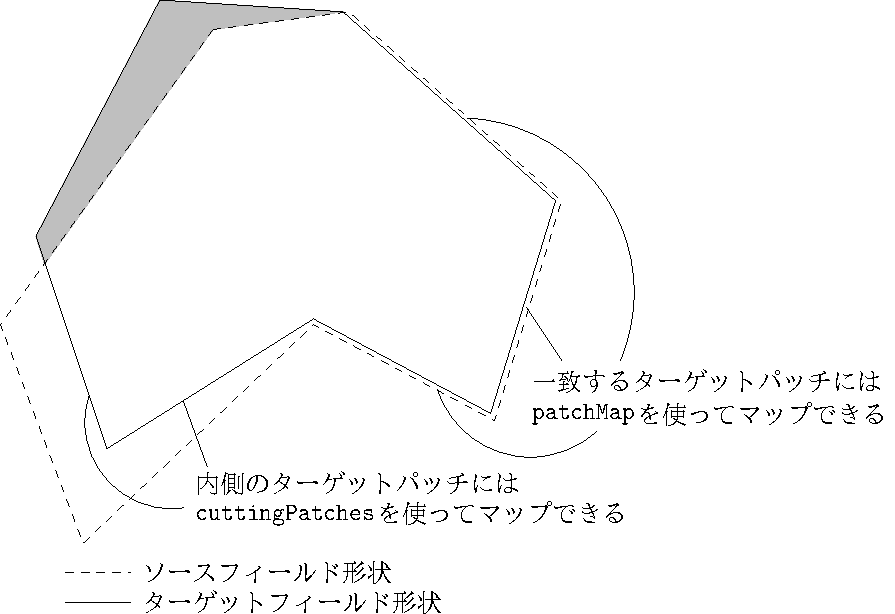
\includegraphics{fig-5-17}
 \caption{一貫しないフィールドをマップする}
 \label{fig:5.17}
\end{figure}

\begin{OFverbatim}[file, linenum=17]

patchMap        ( lid movingWall );

cuttingPatches  ( fixedWalls );


// ************************************************************************* //
\end{OFverbatim}

\begin{OFverbatim}[terminal]
mapFields <source dir>
\end{OFverbatim}


\subsection{並列なケースのマッピング}
\label{ssec:5.6.3}
\OFtool{mapFields}を実行するとき,
並列計算のためにソースとターゲットとなるケースの
どちらかもしくは両方を分解するなら,追加オプションが必要になります.
\begin{description}
 \item[\texttt{-parallelSource}] ソースケースが並列計算のために分解される場合
 \item[\texttt{-parallelTarget}] ターゲットケースが並列計算のために分解される場合
\end{description}
